\section*{Введение}

В данной лабораторной работе рассматриваются двумерные линейные преобразования, задаваемые матрицами $2 \times 2$. Любая такая матрица определяет линейное отображение, преобразующее точки плоскости по закону:

\begin{equation}
\begin{bmatrix} x_{new} \\ y_{new} \end{bmatrix} = 
\begin{bmatrix} a & b \\ c & d \end{bmatrix}
\begin{bmatrix} x_{old} \\ y_{old} \end{bmatrix}
\end{equation}

\subsection*{Подготовка к выполнению заданий}

\subsubsection*{Выбор чисел}

В соответствии с требованиями задания были выбраны четыре различных целых числа, ни одно из которых не равно 0 или $\pm 1$:

\begin{itemize}
\item $a = 3$
\item $b = 5$ 
\item $c = 7$
\item $d = 11$
\end{itemize}

\subsubsection*{Создание многоугольника}

Был создан произвольный шестиугольник с вершинами:
\begin{itemize}
\item $V_1 = (0, 0)$
\item $V_2 = (2, 1)$
\item $V_3 = (3, 3)$
\item $V_4 = (2, 4)$
\item $V_5 = (0, 3)$
\item $V_6 = (-1, 1)$
\end{itemize}

\begin{figure}[h]
\centering
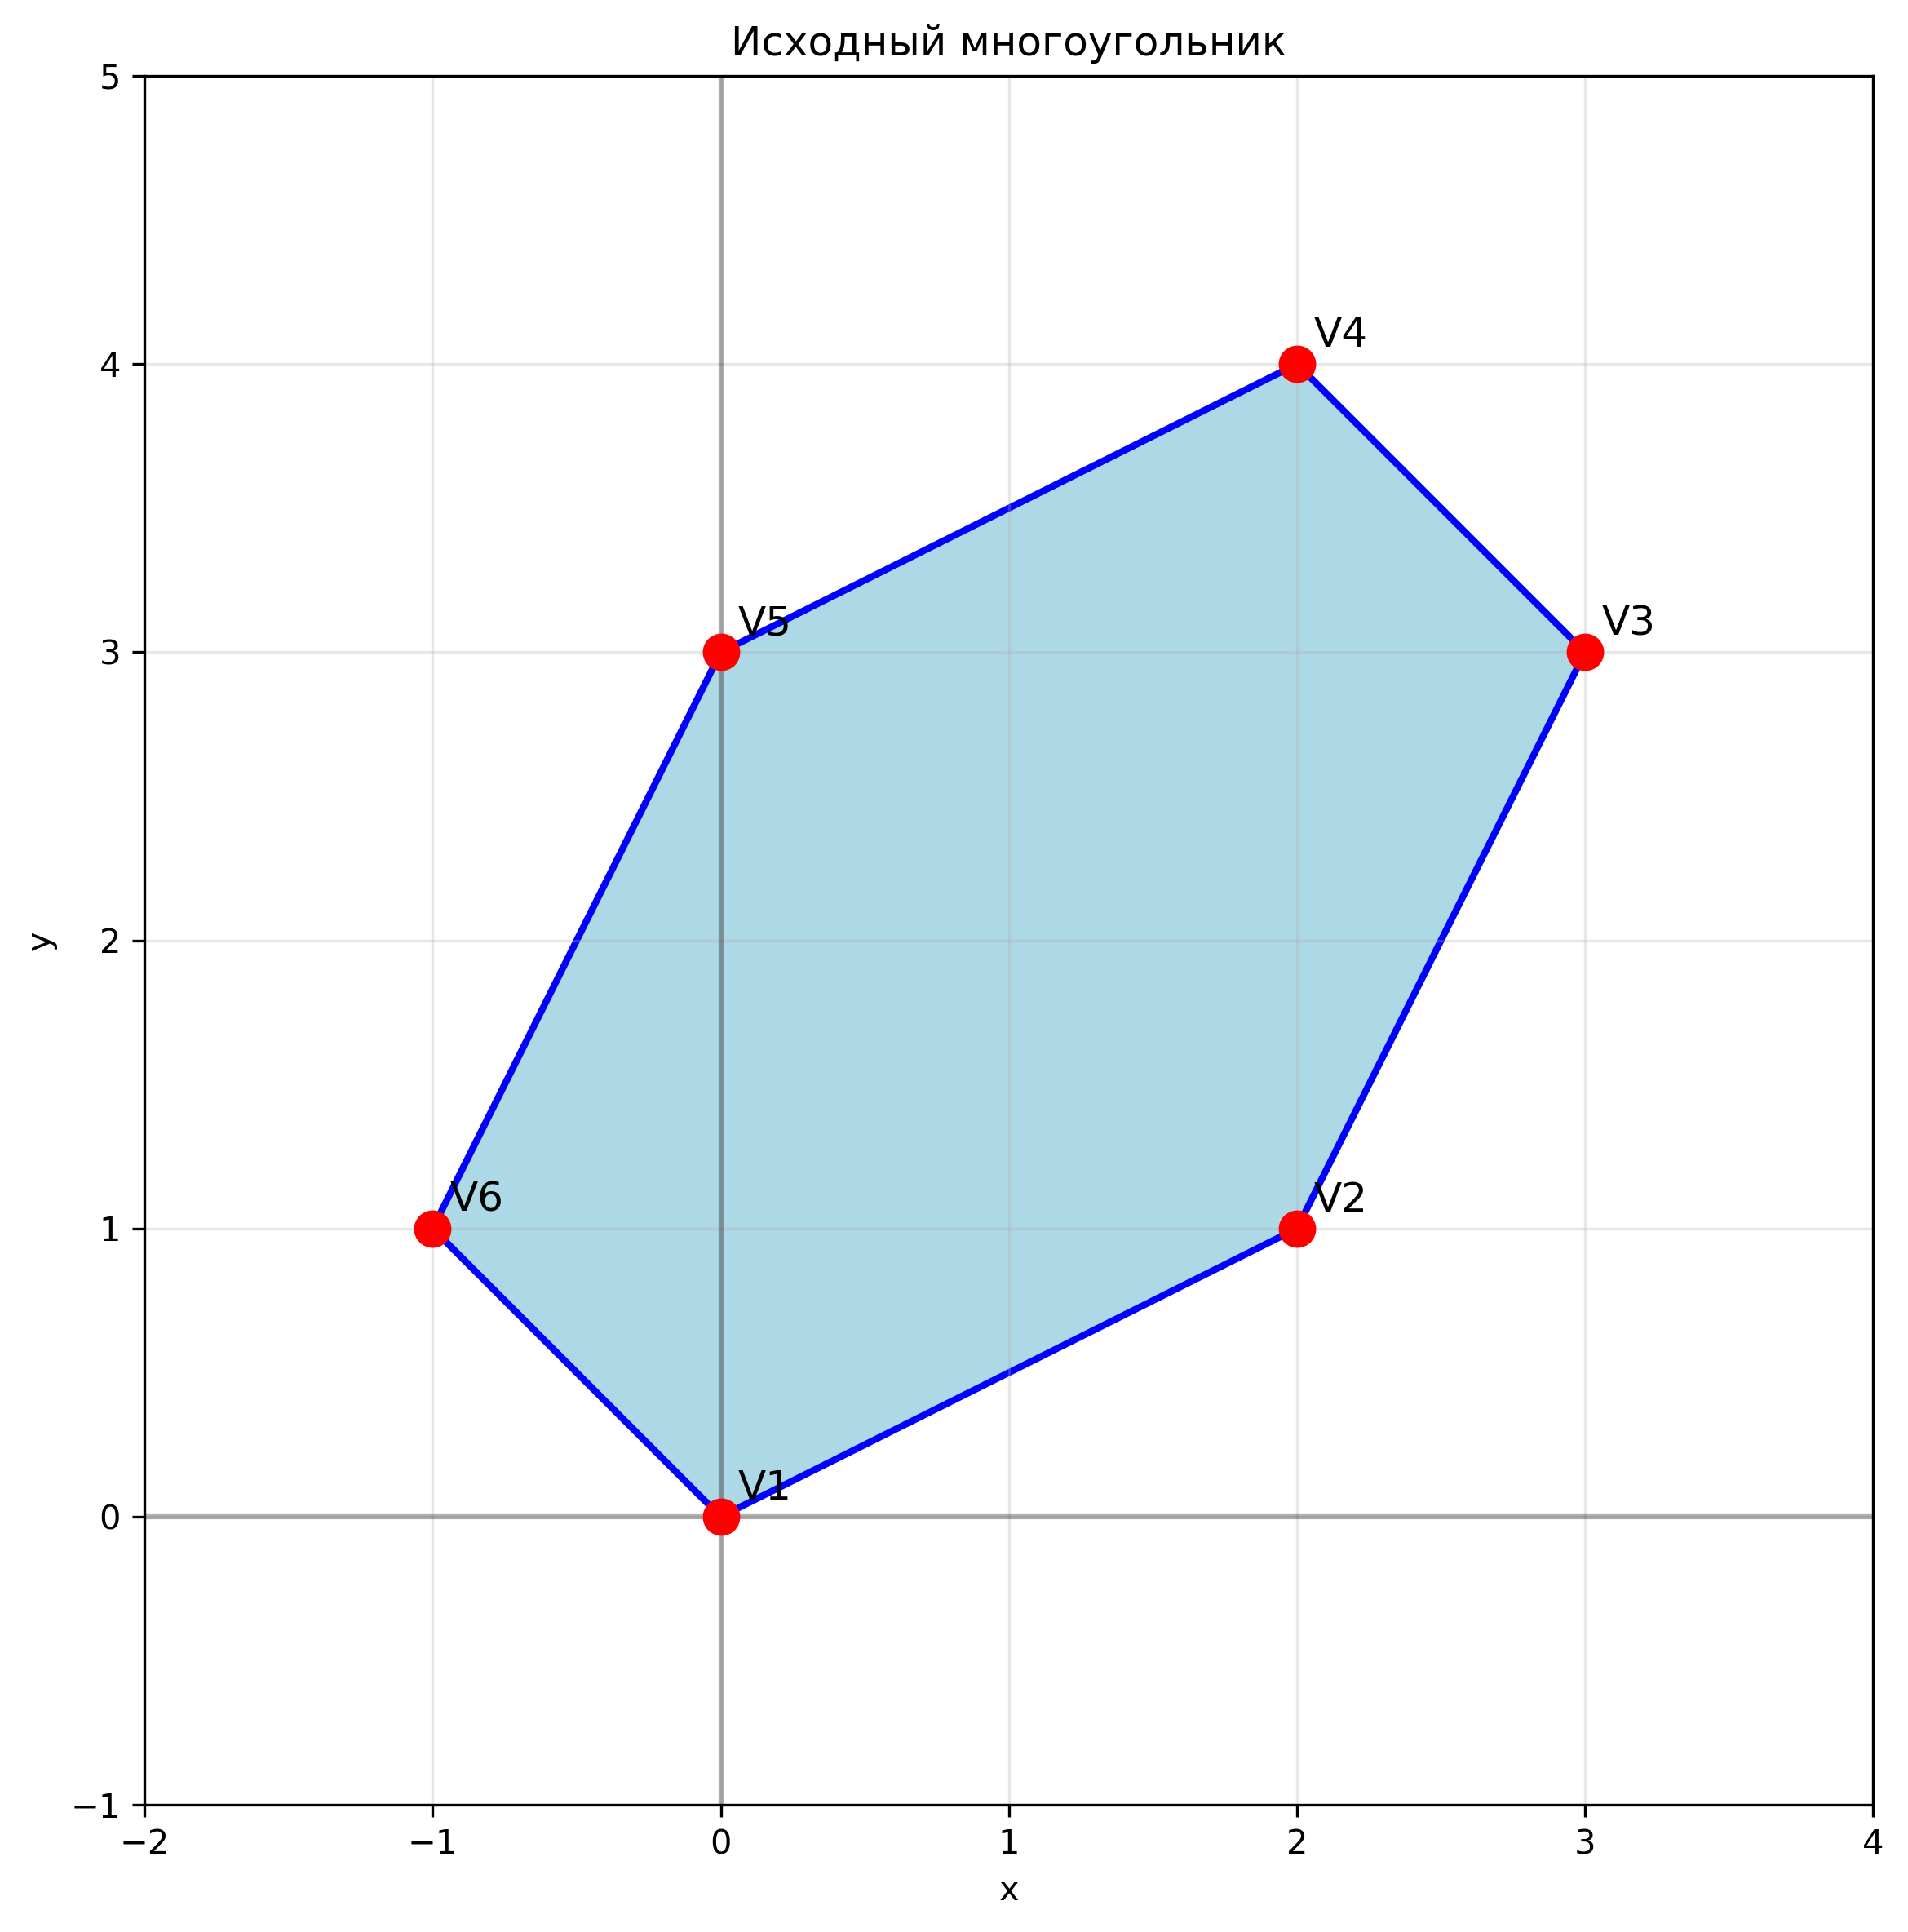
\includegraphics[width=0.6\textwidth]{images/original_polygon.png}
\caption{Исходный многоугольник}
\label{fig:original_polygon}
\end{figure}

Данный многоугольник будет использоваться для визуализации всех матричных преобразований в ходе выполнения заданий.

\section*{Задание 1: Создание матричных преобразований}

В данном разделе будут созданы различные матрицы $2 \times 2$, задающие интересные линейные преобразования плоскости. Для каждого преобразования будет построена соответствующая матрица, вычислены собственные значения и векторы, а также выполнена визуализация преобразования многоугольника.

\subsection*{Отражение относительно прямой $y = ax$}

Матрица отражения относительно прямой $y = 3x$ имеет вид:

\begin{equation}
A_1 = \begin{bmatrix} -0.8 & 0.6 \\ 0.6 & 0.8 \end{bmatrix}
\end{equation}

Собственные значения: $\lambda_1 = -1$, $\lambda_2 = 1$

Собственные векторы:
\begin{itemize}
\item $\lambda_1 = -1$: $\mathbf{v}_1 = \begin{bmatrix} -0.95 \\ 0.32 \end{bmatrix}$
\item $\lambda_2 = 1$: $\mathbf{v}_2 = \begin{bmatrix} -0.32 \\ -0.95 \end{bmatrix}$
\end{itemize}

\begin{figure}[h]
\centering
\begin{minipage}{0.31\textwidth}
\centering
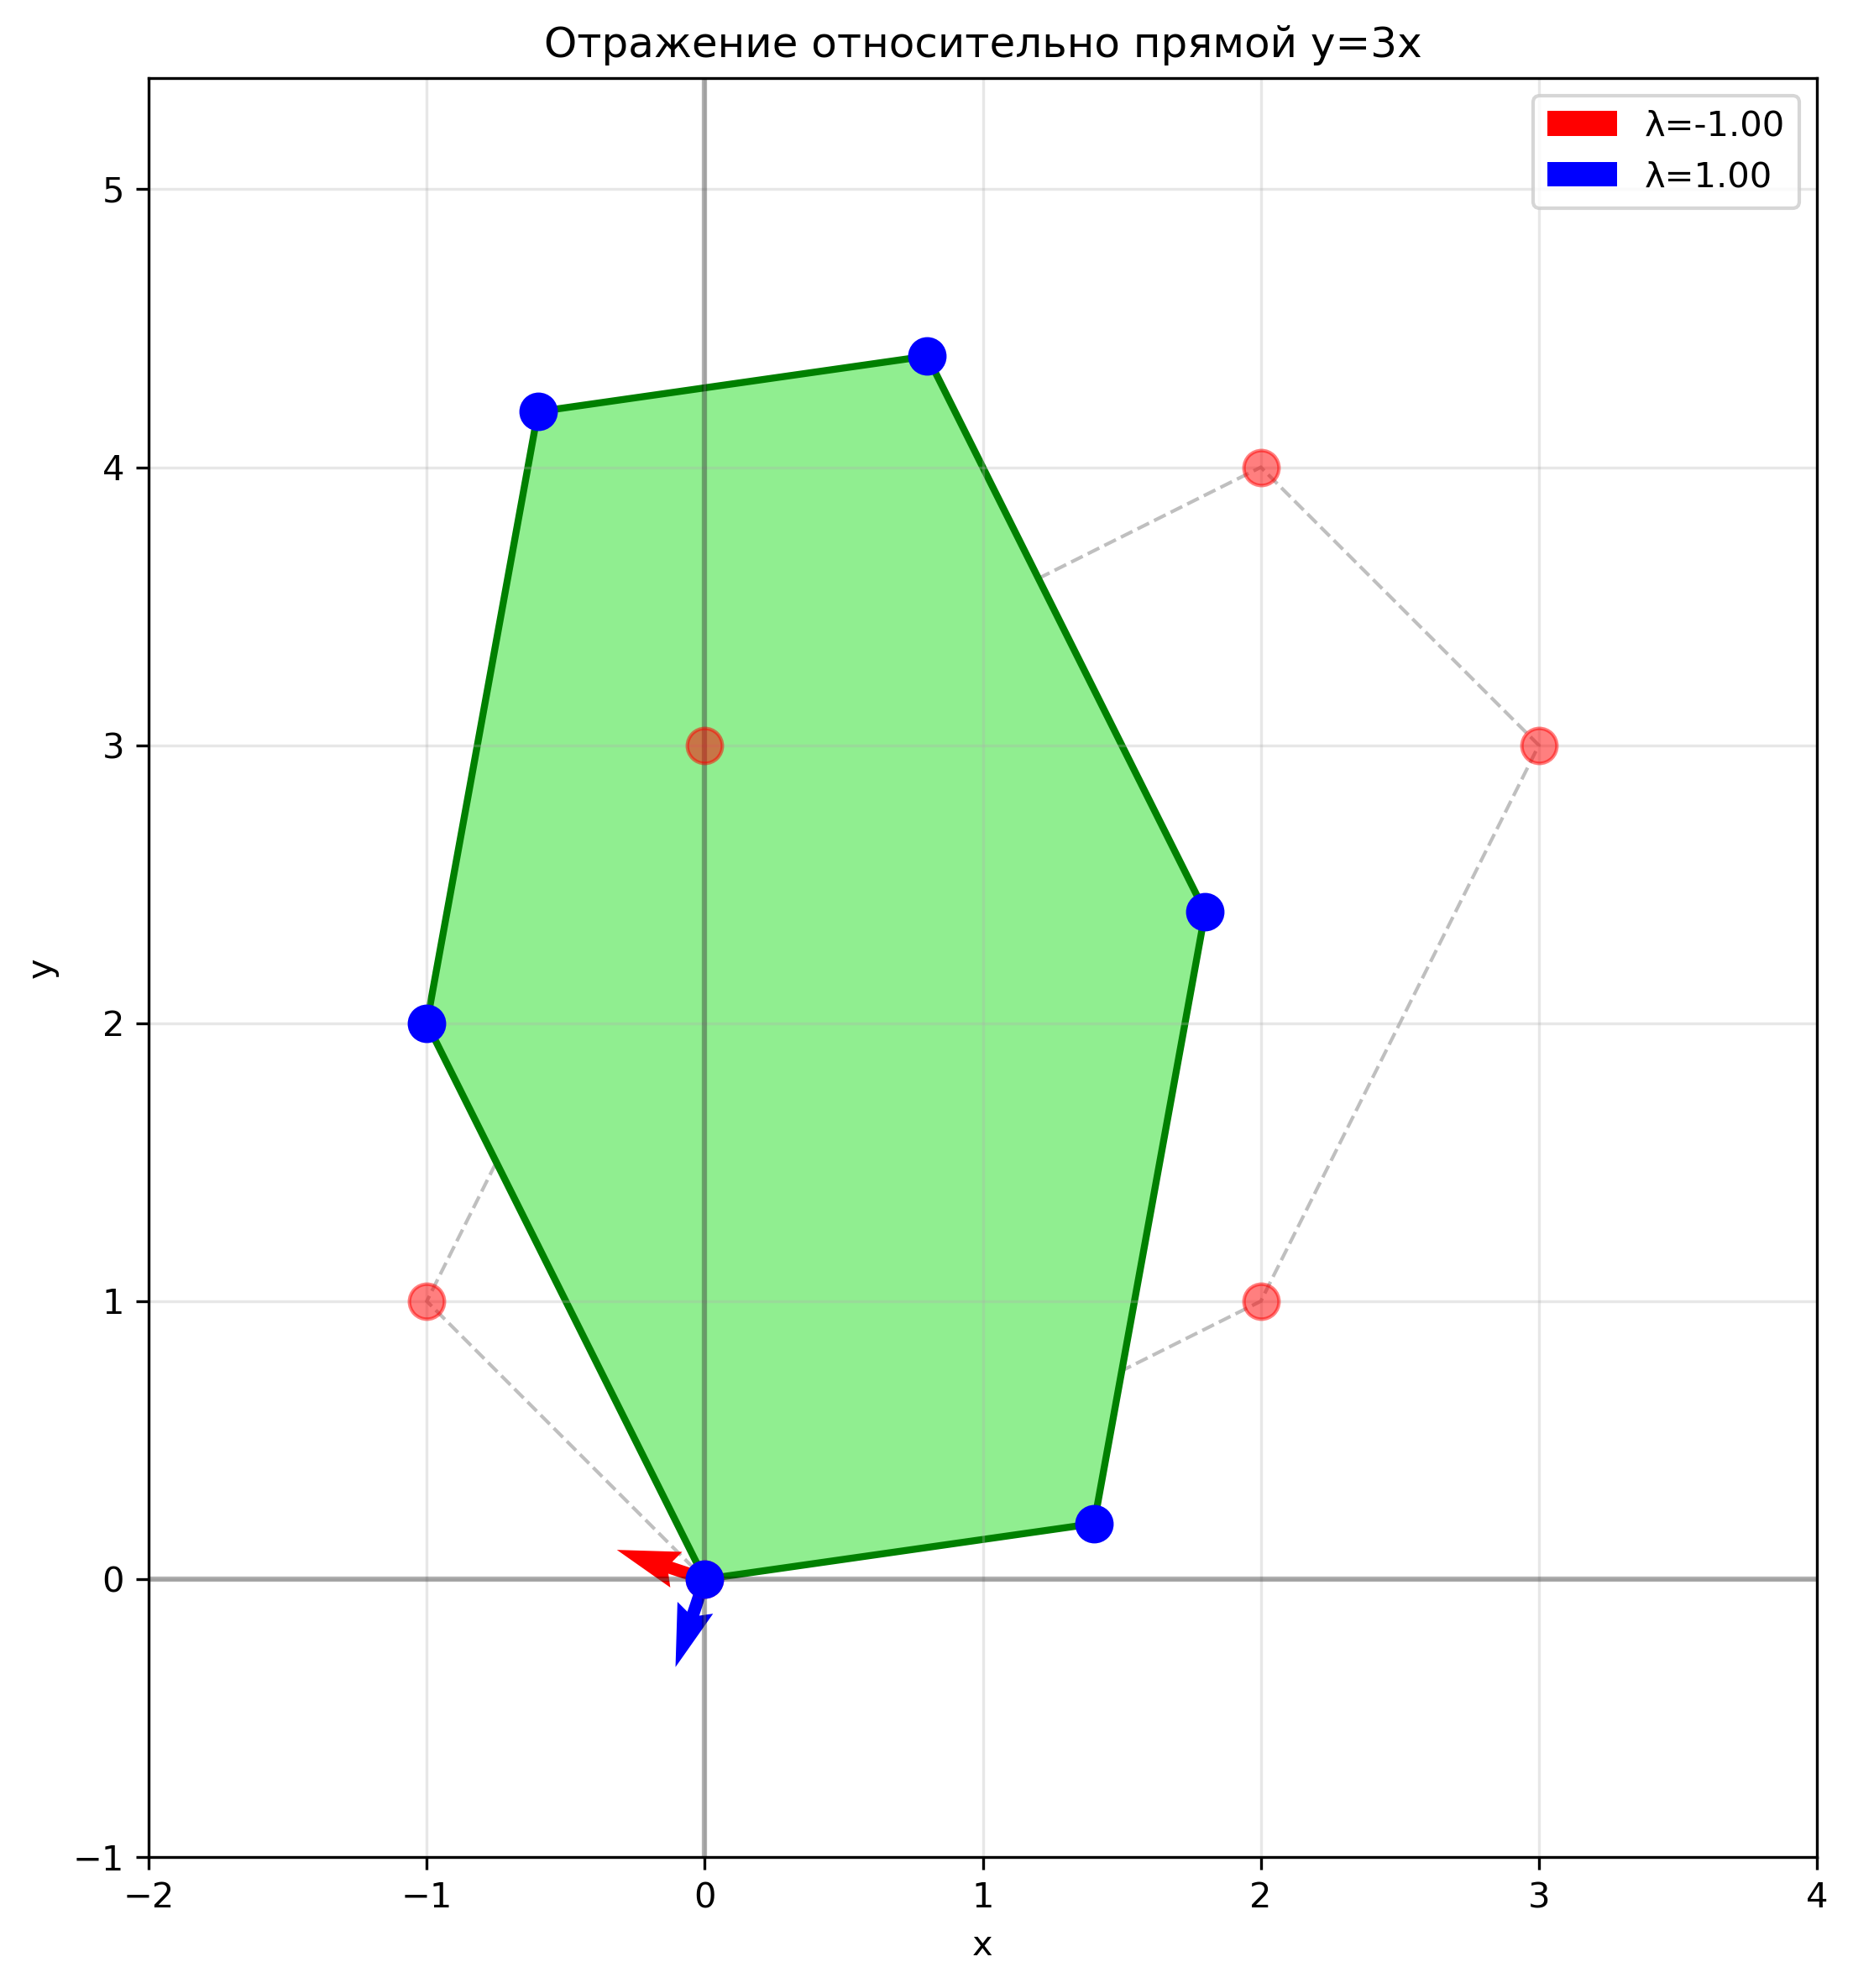
\includegraphics[width=\textwidth]{images/task1/reflection_y_ax.png}
\caption{Отражение относительно прямой $y = 3x$}
\label{fig:reflection_y_ax}
\end{minipage}
\hfill
\begin{minipage}{0.31\textwidth}
\centering
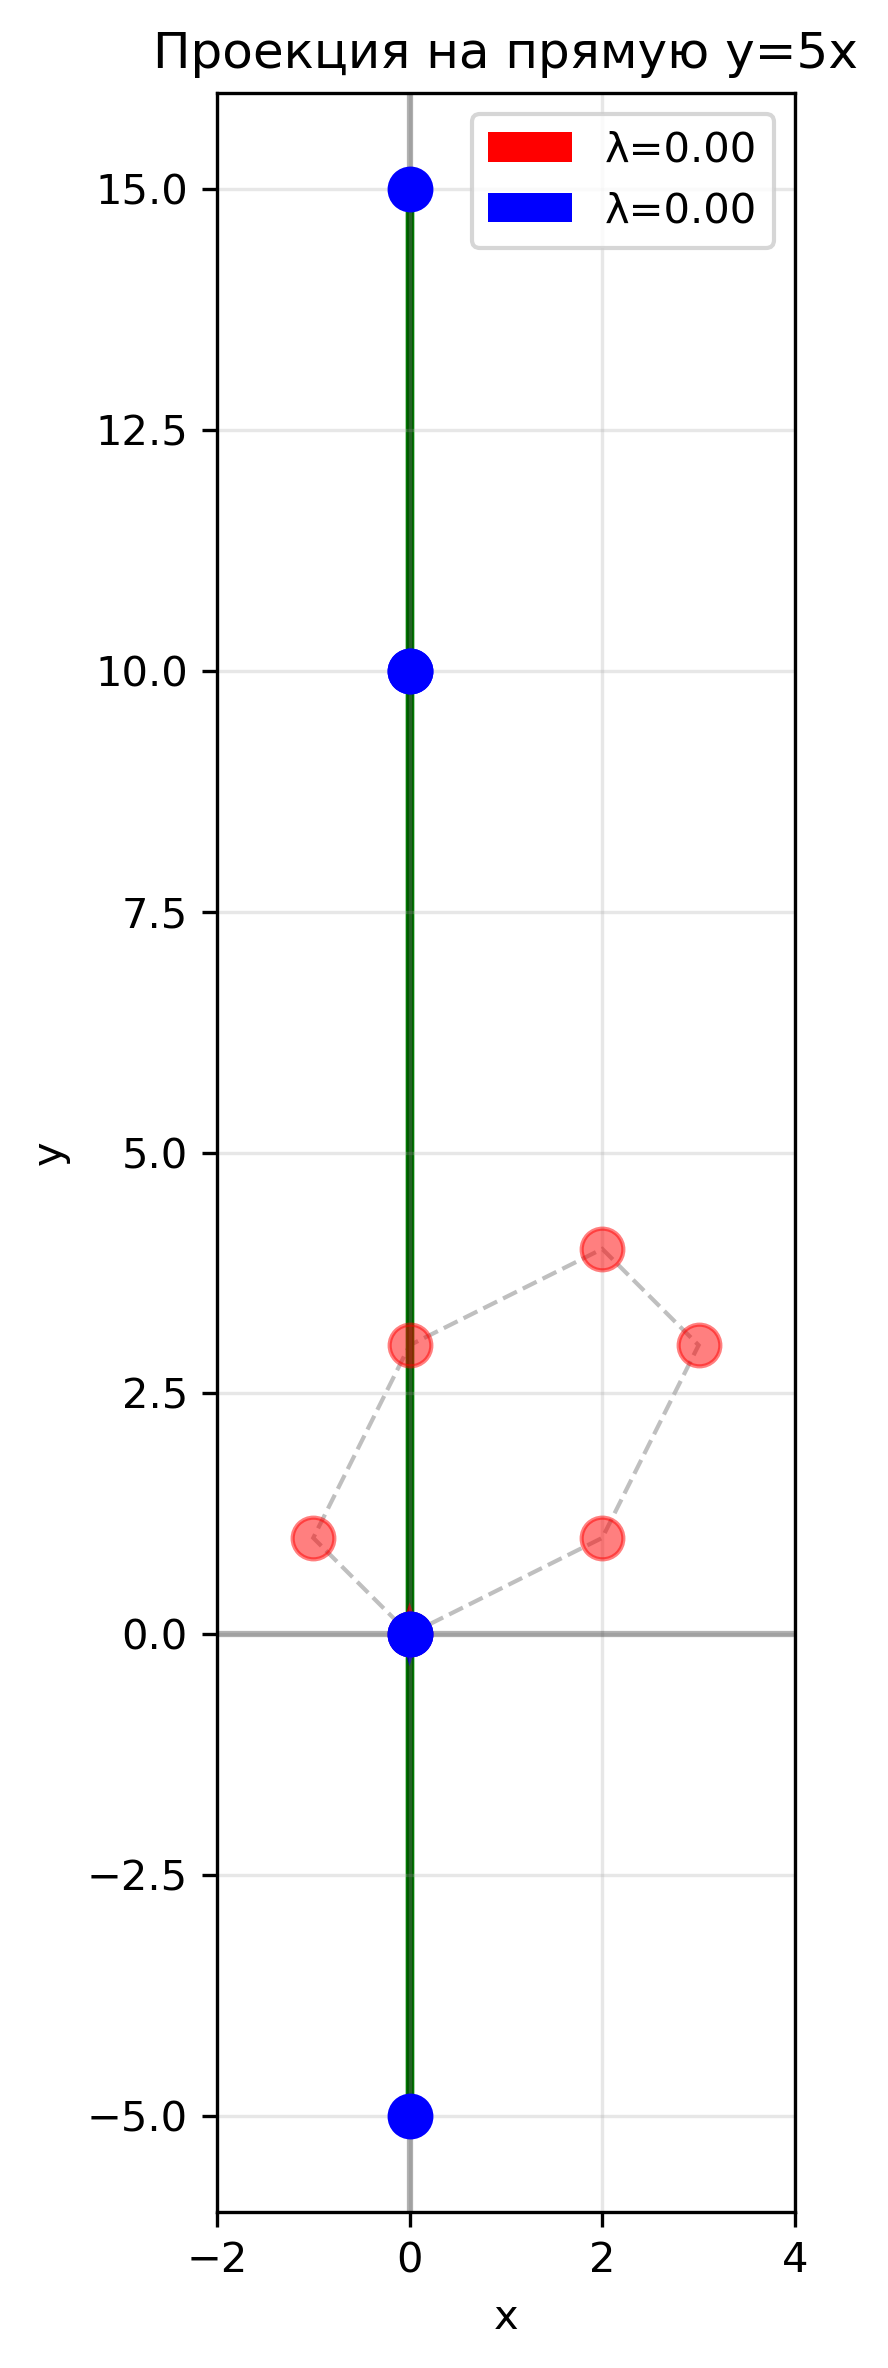
\includegraphics[width=\textwidth]{images/task1/projection_y_bx.png}
\caption{Проекция на прямую $y = 5x$}
\label{fig:projection_y_bx}
\end{minipage}
\hfill
\begin{minipage}{0.31\textwidth}
\centering
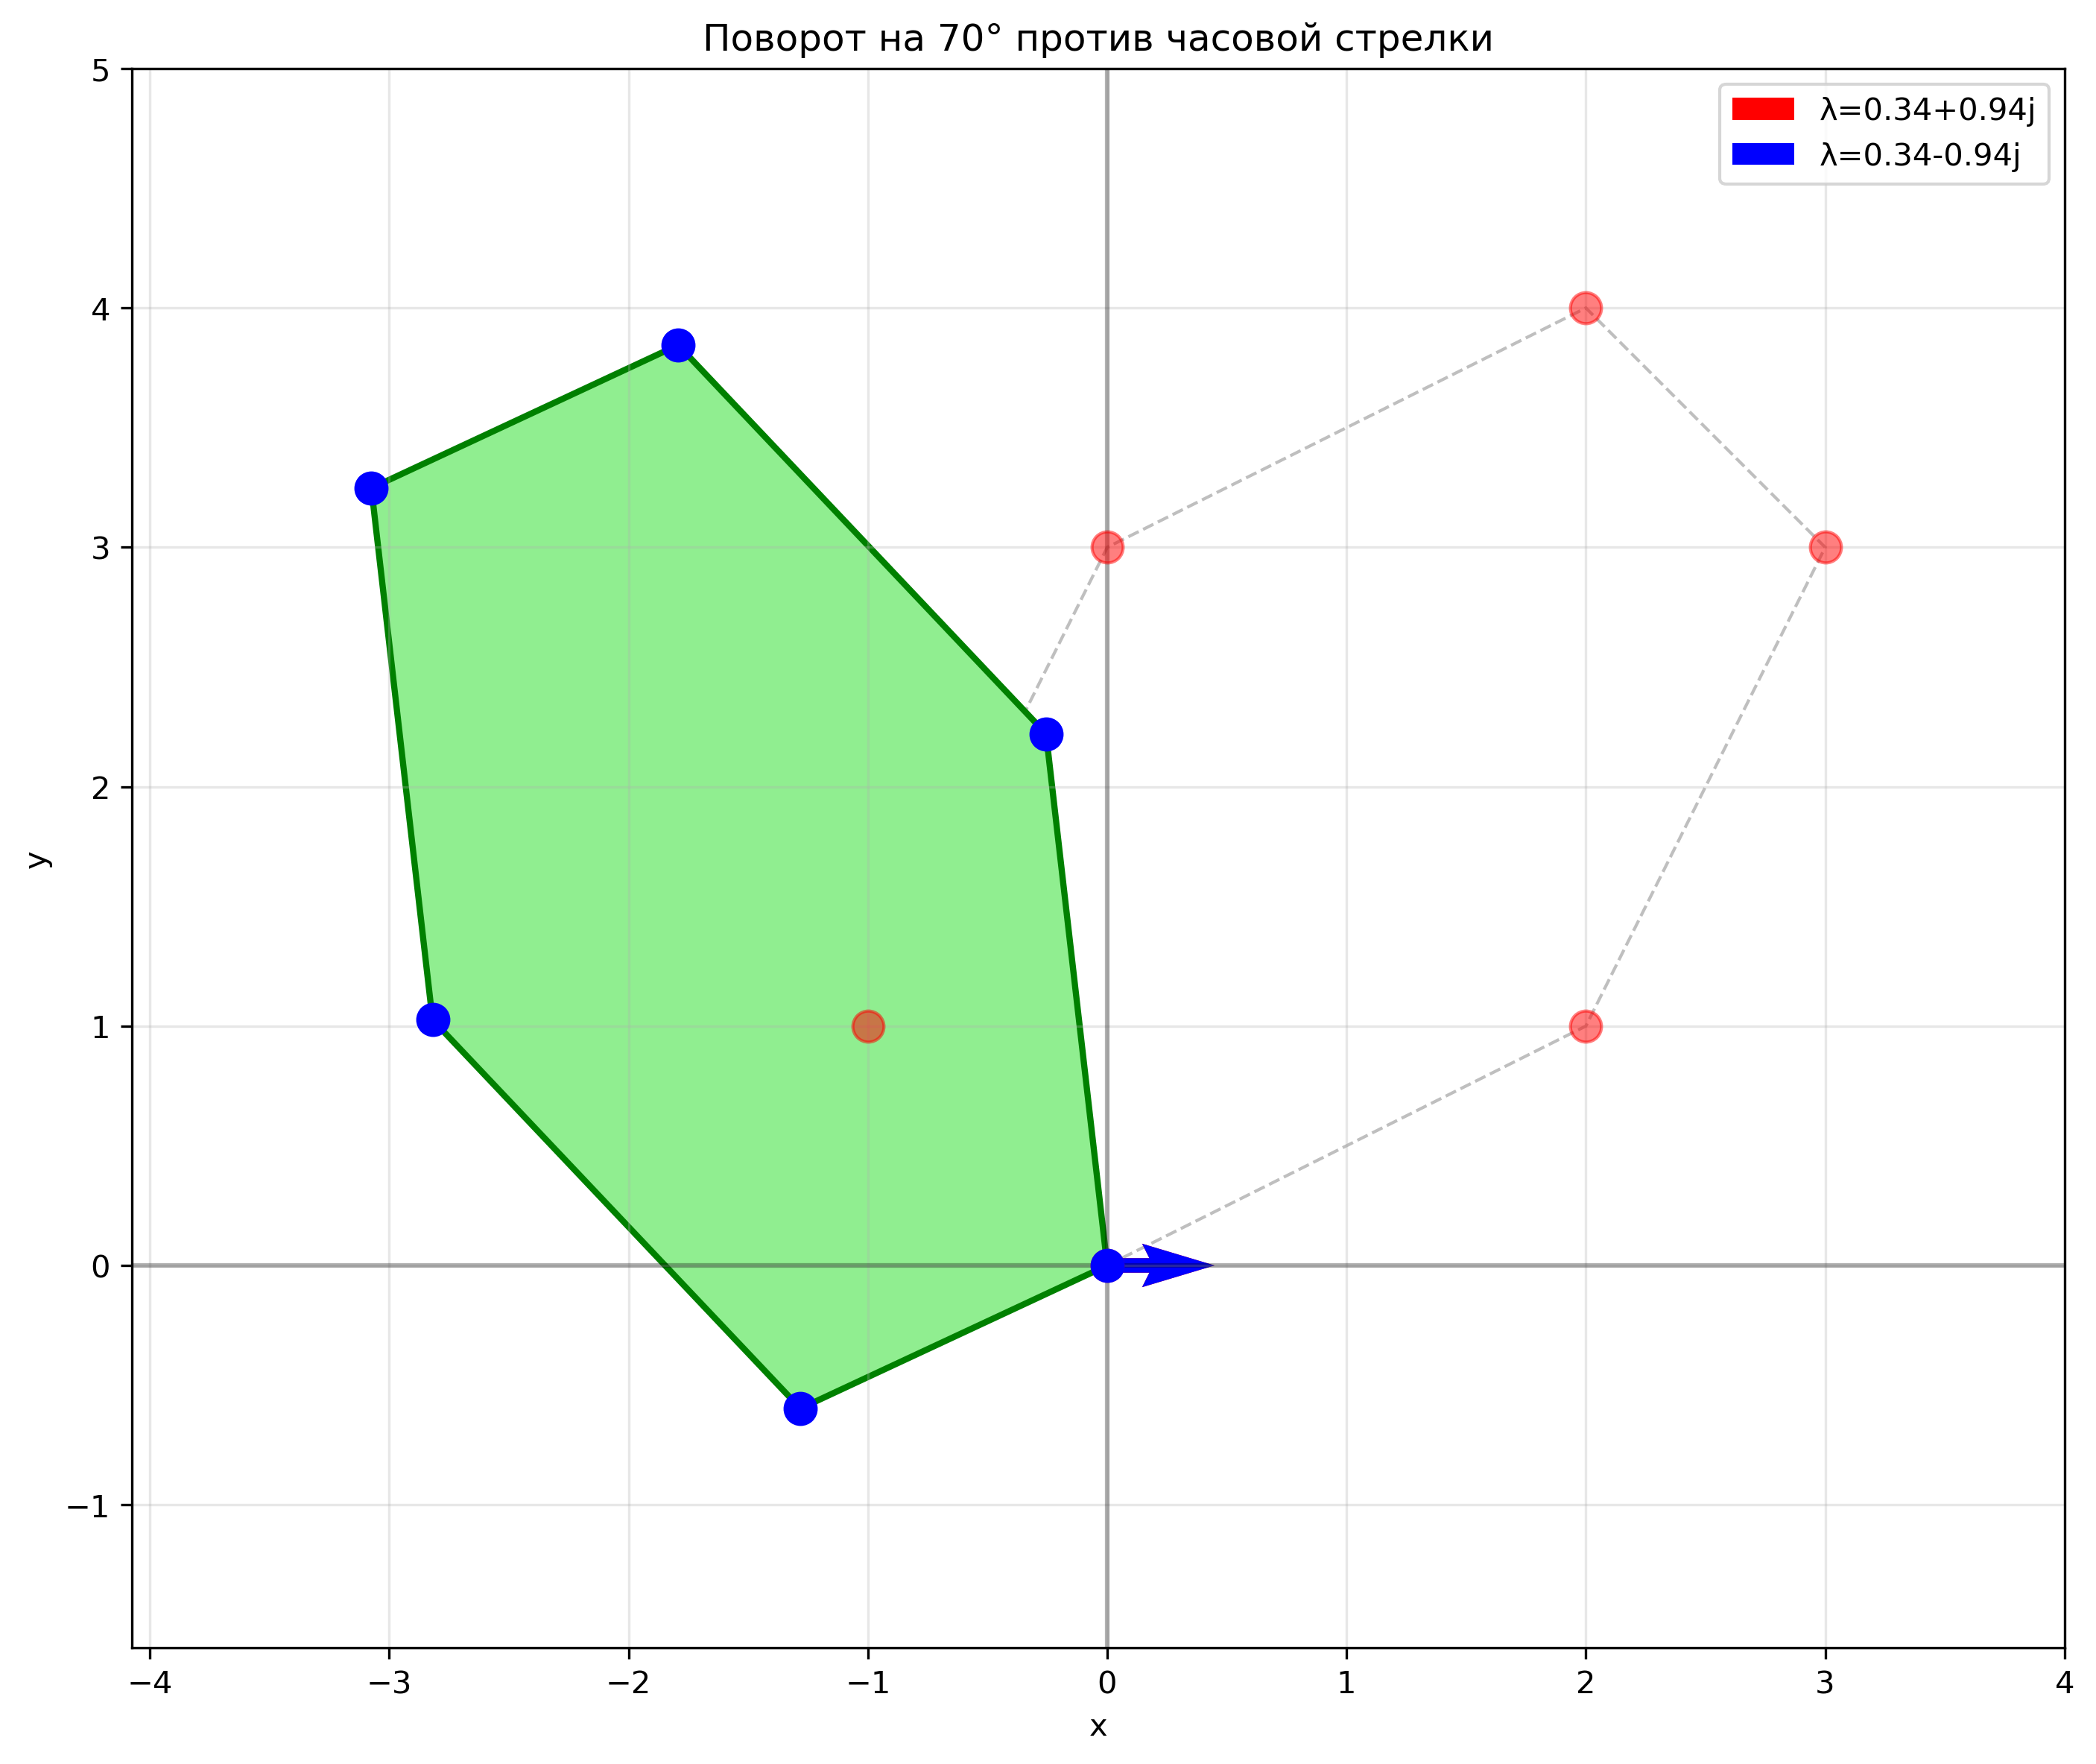
\includegraphics[width=\textwidth]{images/task1/rotation_10c_degrees.png}
\caption{Поворот на $70°$ против часовой стрелки}
\label{fig:rotation_10c_degrees}
\end{minipage}
\end{figure}

\subsection*{Отображение всей плоскости в прямую $y = bx$}

Матрица проекции на прямую $y = 5x$:

\begin{equation}
A_2 = \begin{bmatrix} 0 & 0 \\ 5 & 0 \end{bmatrix}
\end{equation}

Собственные значения: $\lambda_1 = 0$, $\lambda_2 = 0$ (кратное)

Собственные векторы: только один линейно независимый вектор $\begin{bmatrix} 0 \\ 1 \end{bmatrix}$

\subsection*{Поворот плоскости на $10c$ градусов против часовой стрелки}

Матрица поворота на $70°$ (так как $c = 7$):

\begin{equation}
A_3 = \begin{bmatrix} 0.342 & -0.940 \\ 0.940 & 0.342 \end{bmatrix}
\end{equation}

Собственные значения: $\lambda_1 = 0.342 + 0.940i$, $\lambda_2 = 0.342 - 0.940i$ (комплексные)

\subsection*{Центральная симметрия плоскости относительно начала координат}

Матрица центральной симметрии:

\begin{equation}
A_4 = \begin{bmatrix} -1 & 0 \\ 0 & -1 \end{bmatrix}
\end{equation}

Собственные значения: $\lambda_1 = -1$, $\lambda_2 = -1$ (кратное)

\subsection*{Отражение + поворот на $10d$ градусов по часовой стрелке}

Композиция отражения относительно $y = 3x$ и поворота на $110°$ по часовой стрелке:

\begin{equation}
A_5 = \begin{bmatrix} 0.837 & 0.547 \\ 0.547 & -0.837 \end{bmatrix}
\end{equation}

Собственные значения: $\lambda_1 = 1$, $\lambda_2 = -1$

\subsection*{Отображение, переводящее $y = 0$ в $y = ax$ и $x = 0$ в $y = bx$}

Матрица, переводящая базисные векторы:

\begin{equation}
A_6 = \begin{bmatrix} 1 & 3 \\ 0 & 5 \end{bmatrix}
\end{equation}

Собственные значения: $\lambda_1 = 1$, $\lambda_2 = 5$

\subsection*{Отображение, переводящее $y = ax$ в $y = 0$ и $y = bx$ в $x = 0$}

Обратная матрица к предыдущей:

\begin{equation}
A_7 = \begin{bmatrix} 1 & -0.6 \\ 0 & 0.2 \end{bmatrix}
\end{equation}

Собственные значения: $\lambda_1 = 1$, $\lambda_2 = 0.2$

\subsection*{Отображение, меняющее местами прямые $y = ax$ и $y = bx$}

Матрица обмена прямых:

\begin{equation}
A_8 = \begin{bmatrix} 1.667 & 0 \\ 0 & 0.6 \end{bmatrix}
\end{equation}

Собственные значения: $\lambda_1 = 1.667$, $\lambda_2 = 0.6$

\begin{figure}[h]
\centering
\begin{minipage}{0.31\textwidth}
\centering
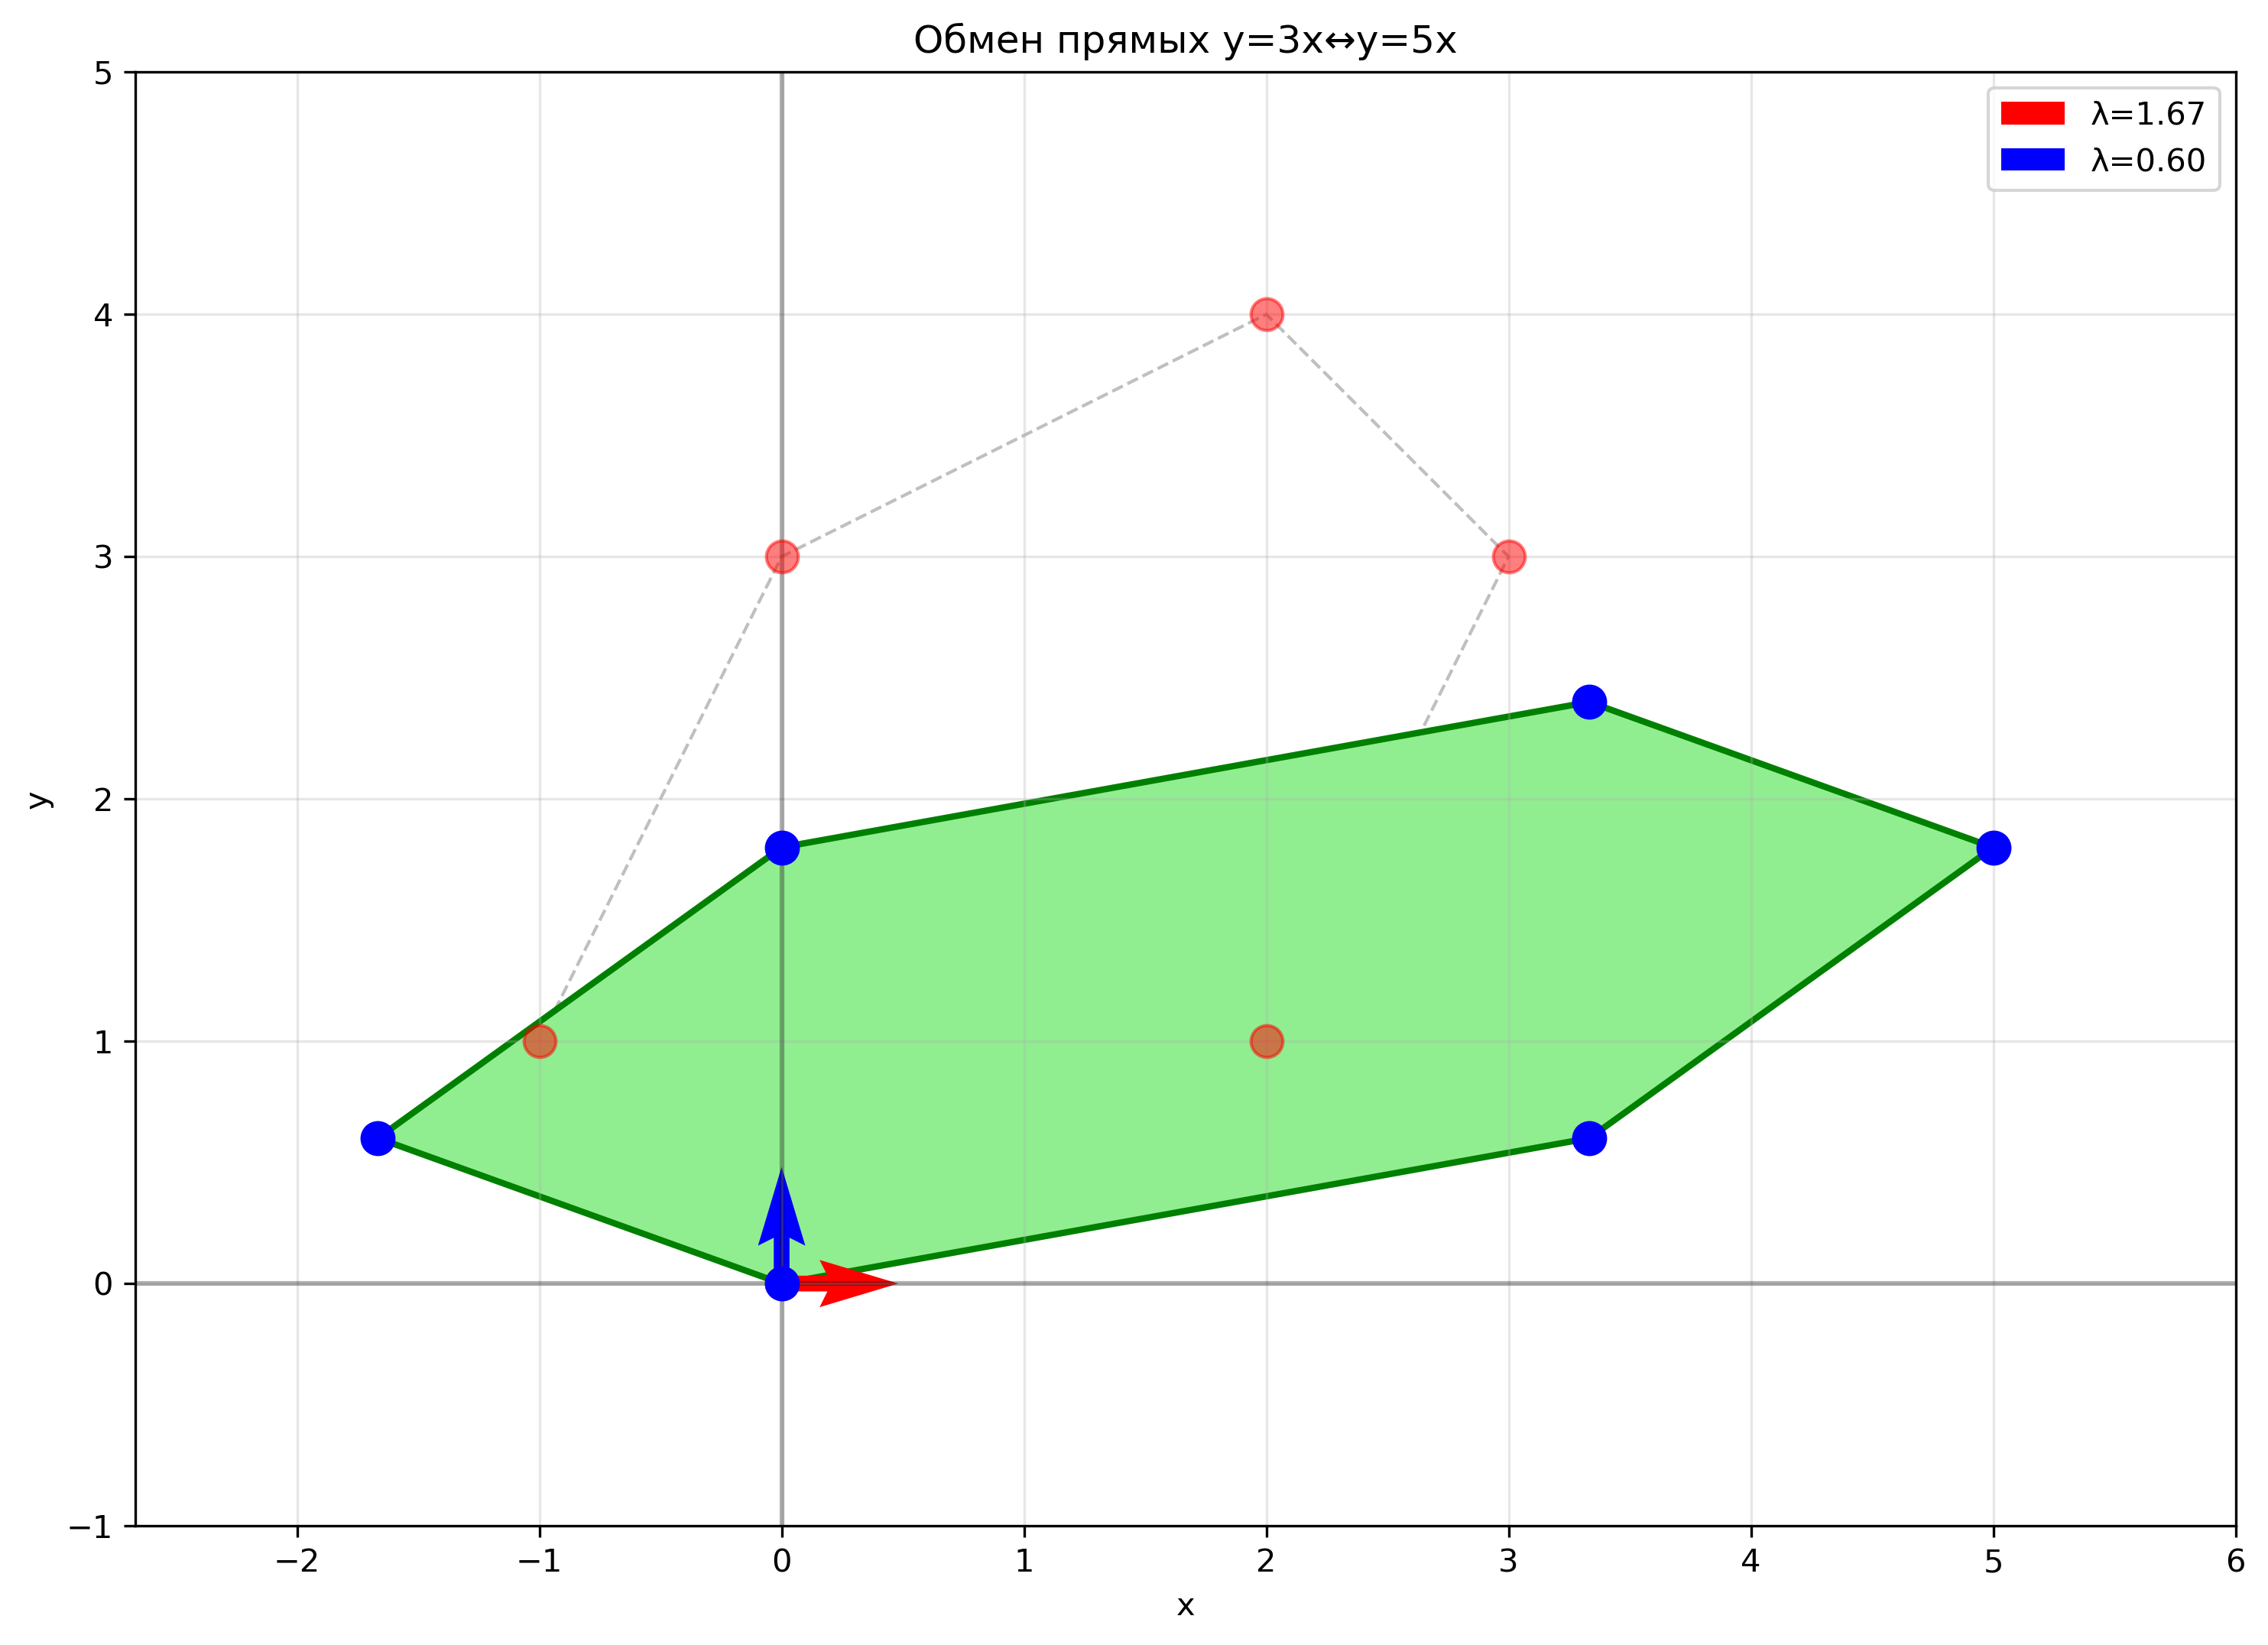
\includegraphics[width=\textwidth]{images/task1/transformation_8.png}
\caption{Обмен прямых $y = 3x \leftrightarrow y = 5x$}
\label{fig:transformation_8}
\end{minipage}
\hfill
\begin{minipage}{0.31\textwidth}
\centering
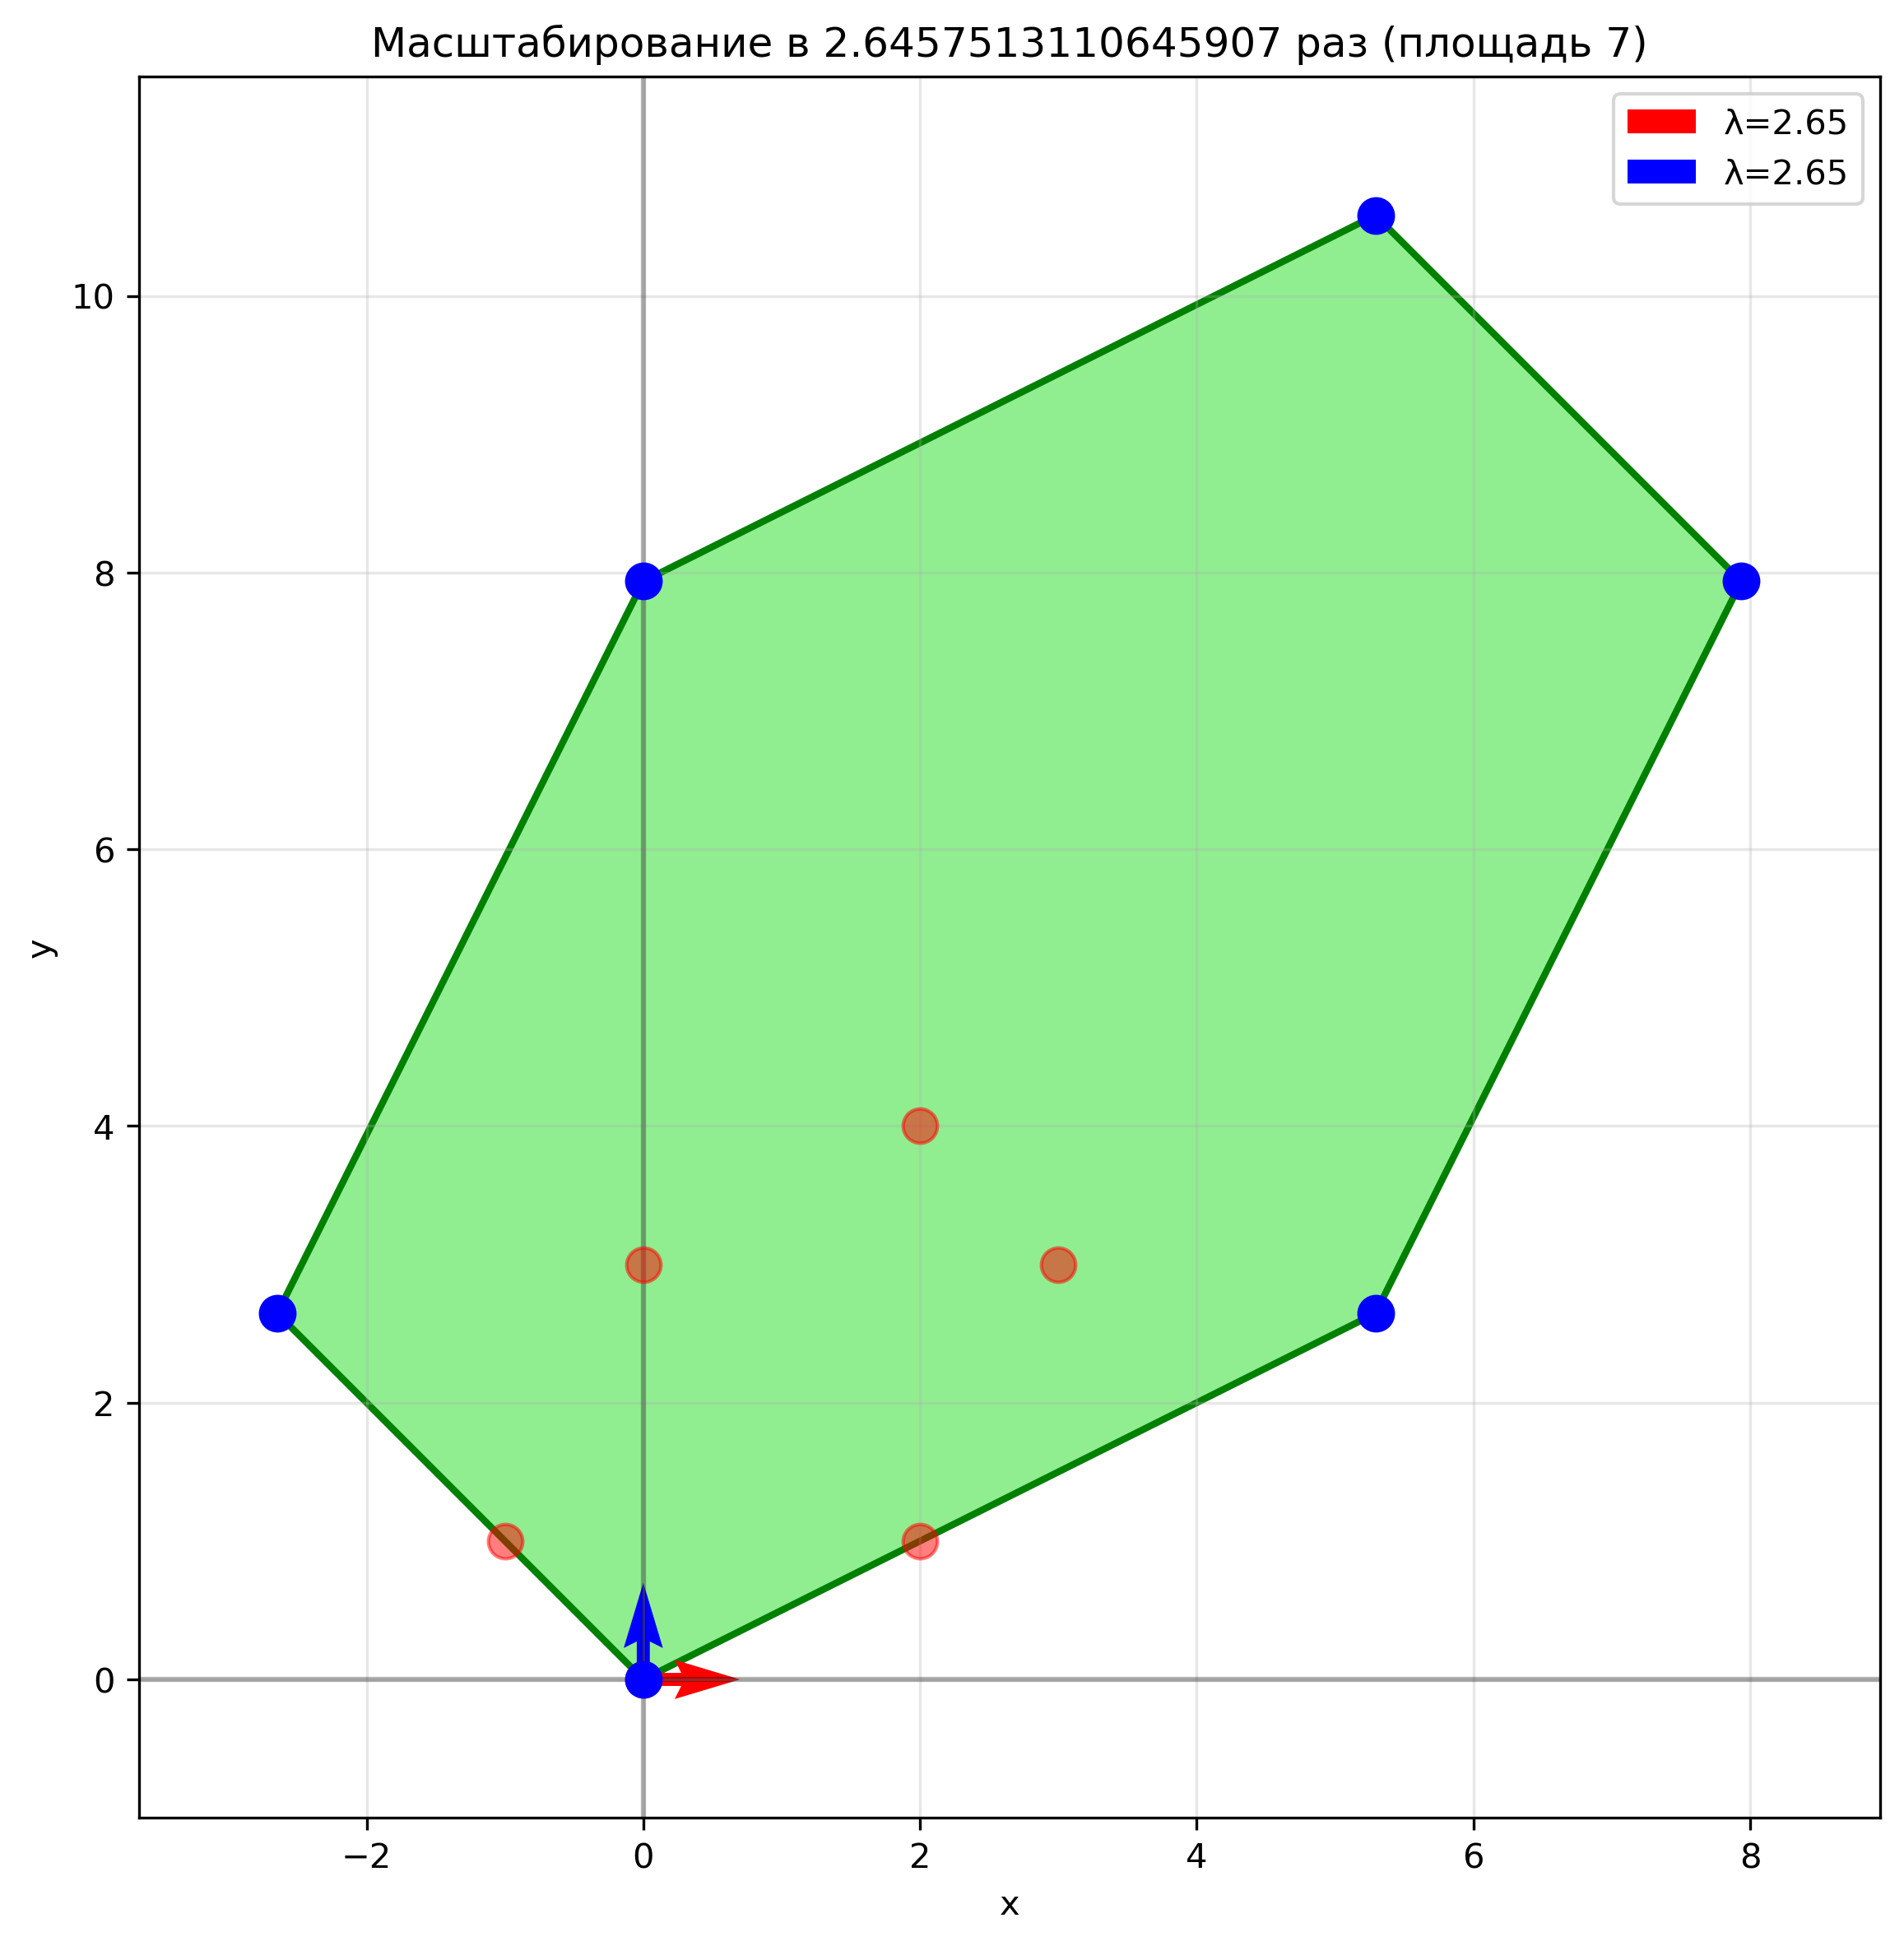
\includegraphics[width=\textwidth]{images/task1/scaling_c.png}
\caption{Масштабирование в $2.646$ раз (площадь $7$)}
\label{fig:scaling_c}
\end{minipage}
\hfill
\begin{minipage}{0.31\textwidth}
\centering
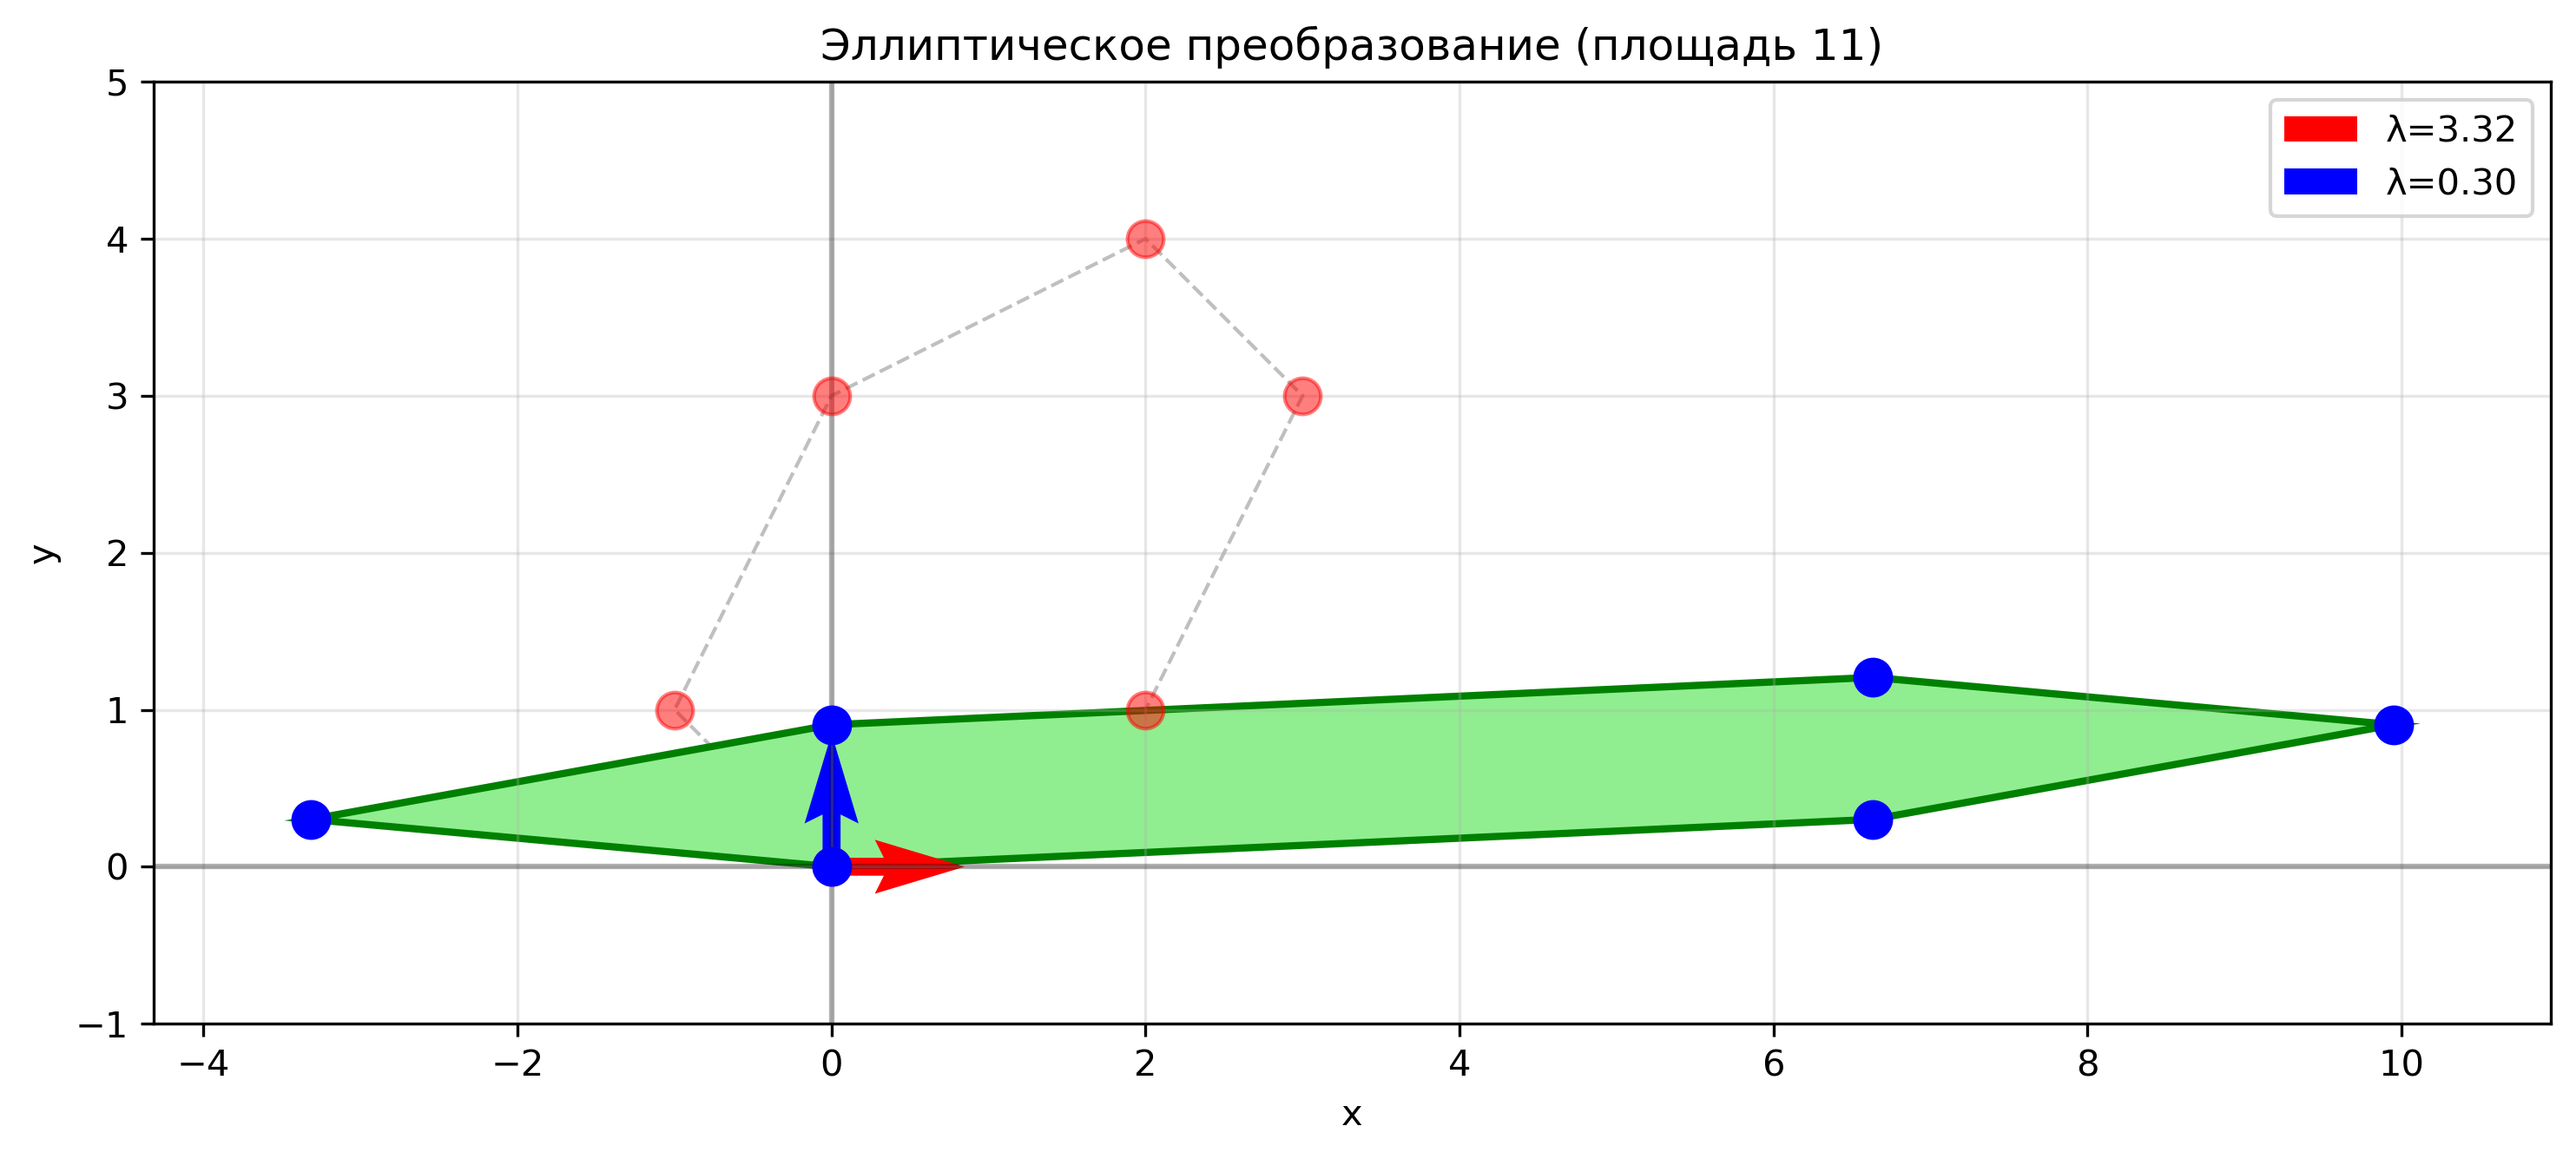
\includegraphics[width=\textwidth]{images/task1/elliptic_d.png}
\caption{Эллиптическое преобразование (площадь $11$)}
\label{fig:elliptic_d}
\end{minipage}
\end{figure}

\subsection*{Отображение, переводящее круг единичной площади в круг площади $c$}

Масштабирование с коэффициентом $\sqrt{7} \approx 2.646$:

\begin{equation}
A_9 = \begin{bmatrix} 2.646 & 0 \\ 0 & 2.646 \end{bmatrix}
\end{equation}

Собственные значения: $\lambda_1 = 2.646$, $\lambda_2 = 2.646$ (кратное)

\subsection*{Отображение, переводящее круг единичной площади в некруг площади $d$}

Эллиптическое преобразование:

\begin{equation}
A_{10} = \begin{bmatrix} 3.317 & 0 \\ 0 & 0.302 \end{bmatrix}
\end{equation}

Собственные значения: $\lambda_1 = 3.317$, $\lambda_2 = 0.302$

\subsection*{Отображение с перпендикулярными собственными векторами}

Симметричная матрица:

\begin{equation}
A_{11} = \begin{bmatrix} 2 & 1 \\ 1 & 3 \end{bmatrix}
\end{equation}

Собственные значения: $\lambda_1 = 1.382$, $\lambda_2 = 3.618$

\subsection*{Отображение без двух неколлинеарных собственных векторов}

Матрица с кратным собственным значением:

\begin{equation}
A_{12} = \begin{bmatrix} 2 & 1 \\ 0 & 2 \end{bmatrix}
\end{equation}

Собственные значения: $\lambda_1 = 2$, $\lambda_2 = 2$ (кратное)

\subsection*{Отображение без вещественных собственных векторов}

Матрица с комплексными собственными значениями:

\begin{equation}
A_{13} = \begin{bmatrix} 0 & -1 \\ 1 & 0 \end{bmatrix}
\end{equation}

Собственные значения: $\lambda_1 = i$, $\lambda_2 = -i$ (чисто мнимые)

\subsection*{Отображение, для которого любой ненулевой вектор является собственным}

Скалярная матрица:

\begin{equation}
A_{14} = \begin{bmatrix} 2 & 0 \\ 0 & 2 \end{bmatrix}
\end{equation}

Собственные значения: $\lambda_1 = 2$, $\lambda_2 = 2$ (кратное)

\begin{figure}[h]
\centering
\begin{minipage}{0.31\textwidth}
\centering
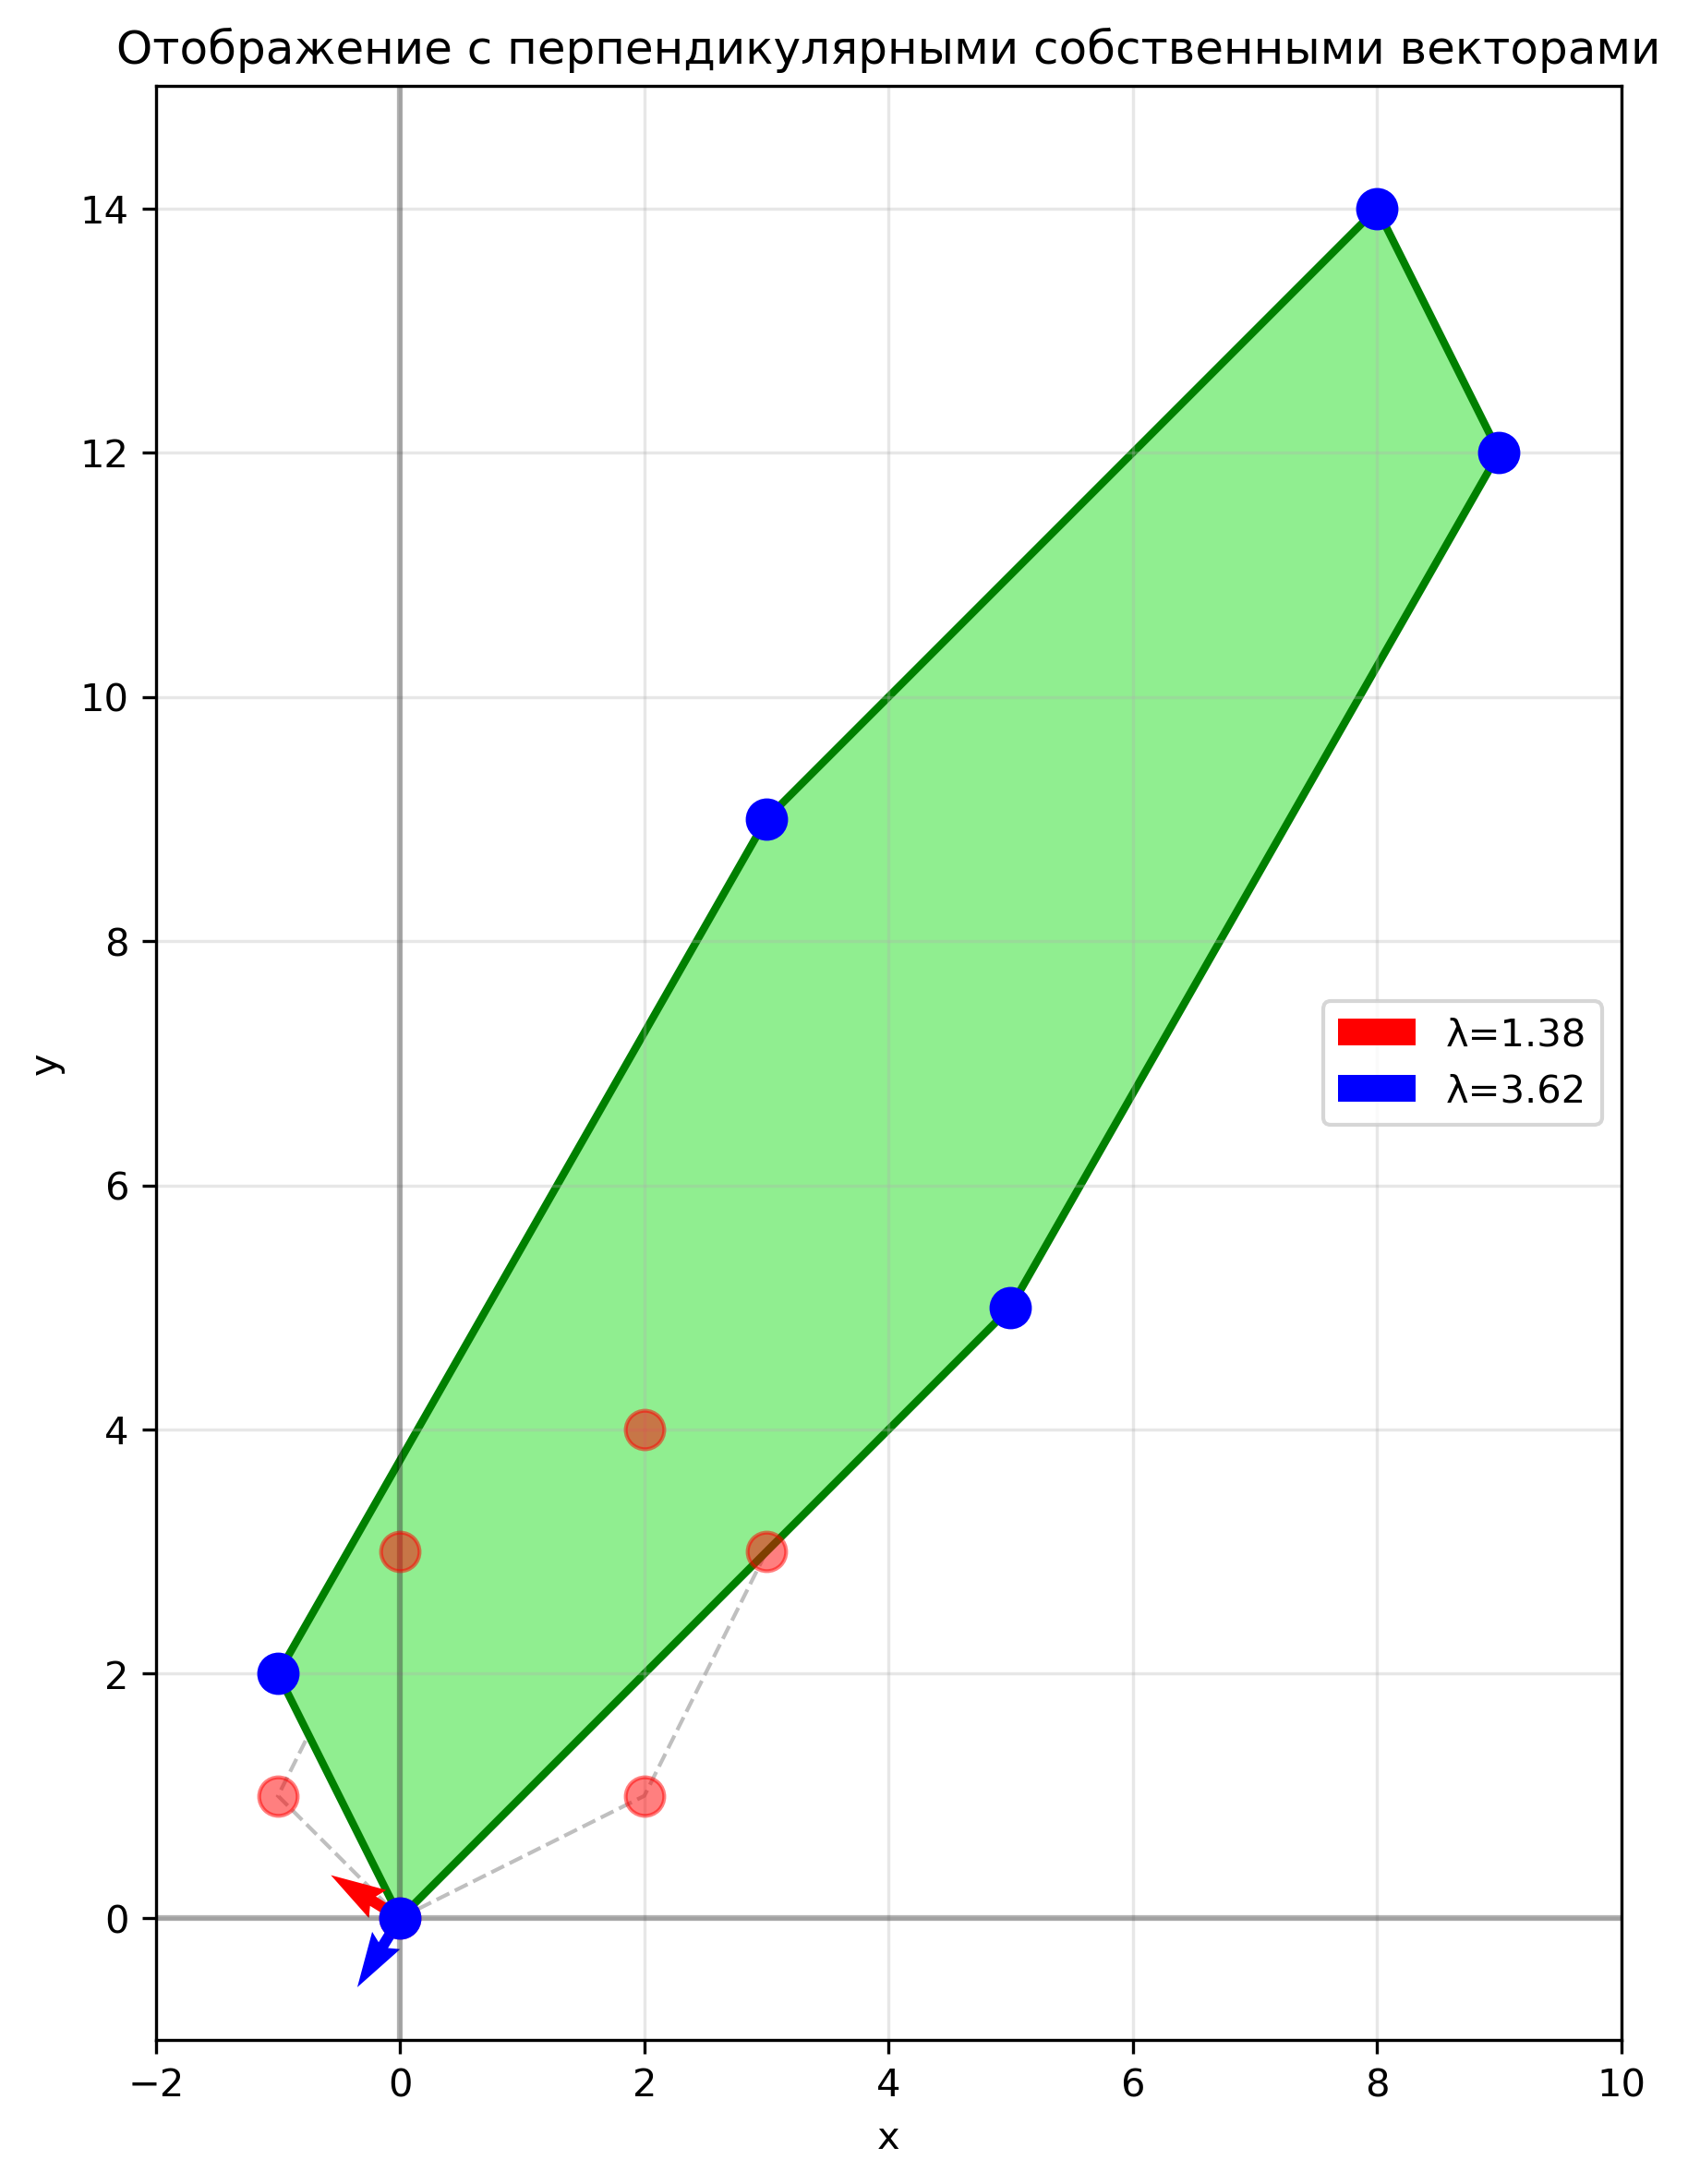
\includegraphics[width=\textwidth]{images/task1/perpendicular_eigenvectors.png}
\caption{Отображение с перпендикулярными собственными векторами}
\label{fig:perpendicular_eigenvectors}
\end{minipage}
\hfill
\begin{minipage}{0.31\textwidth}
\centering
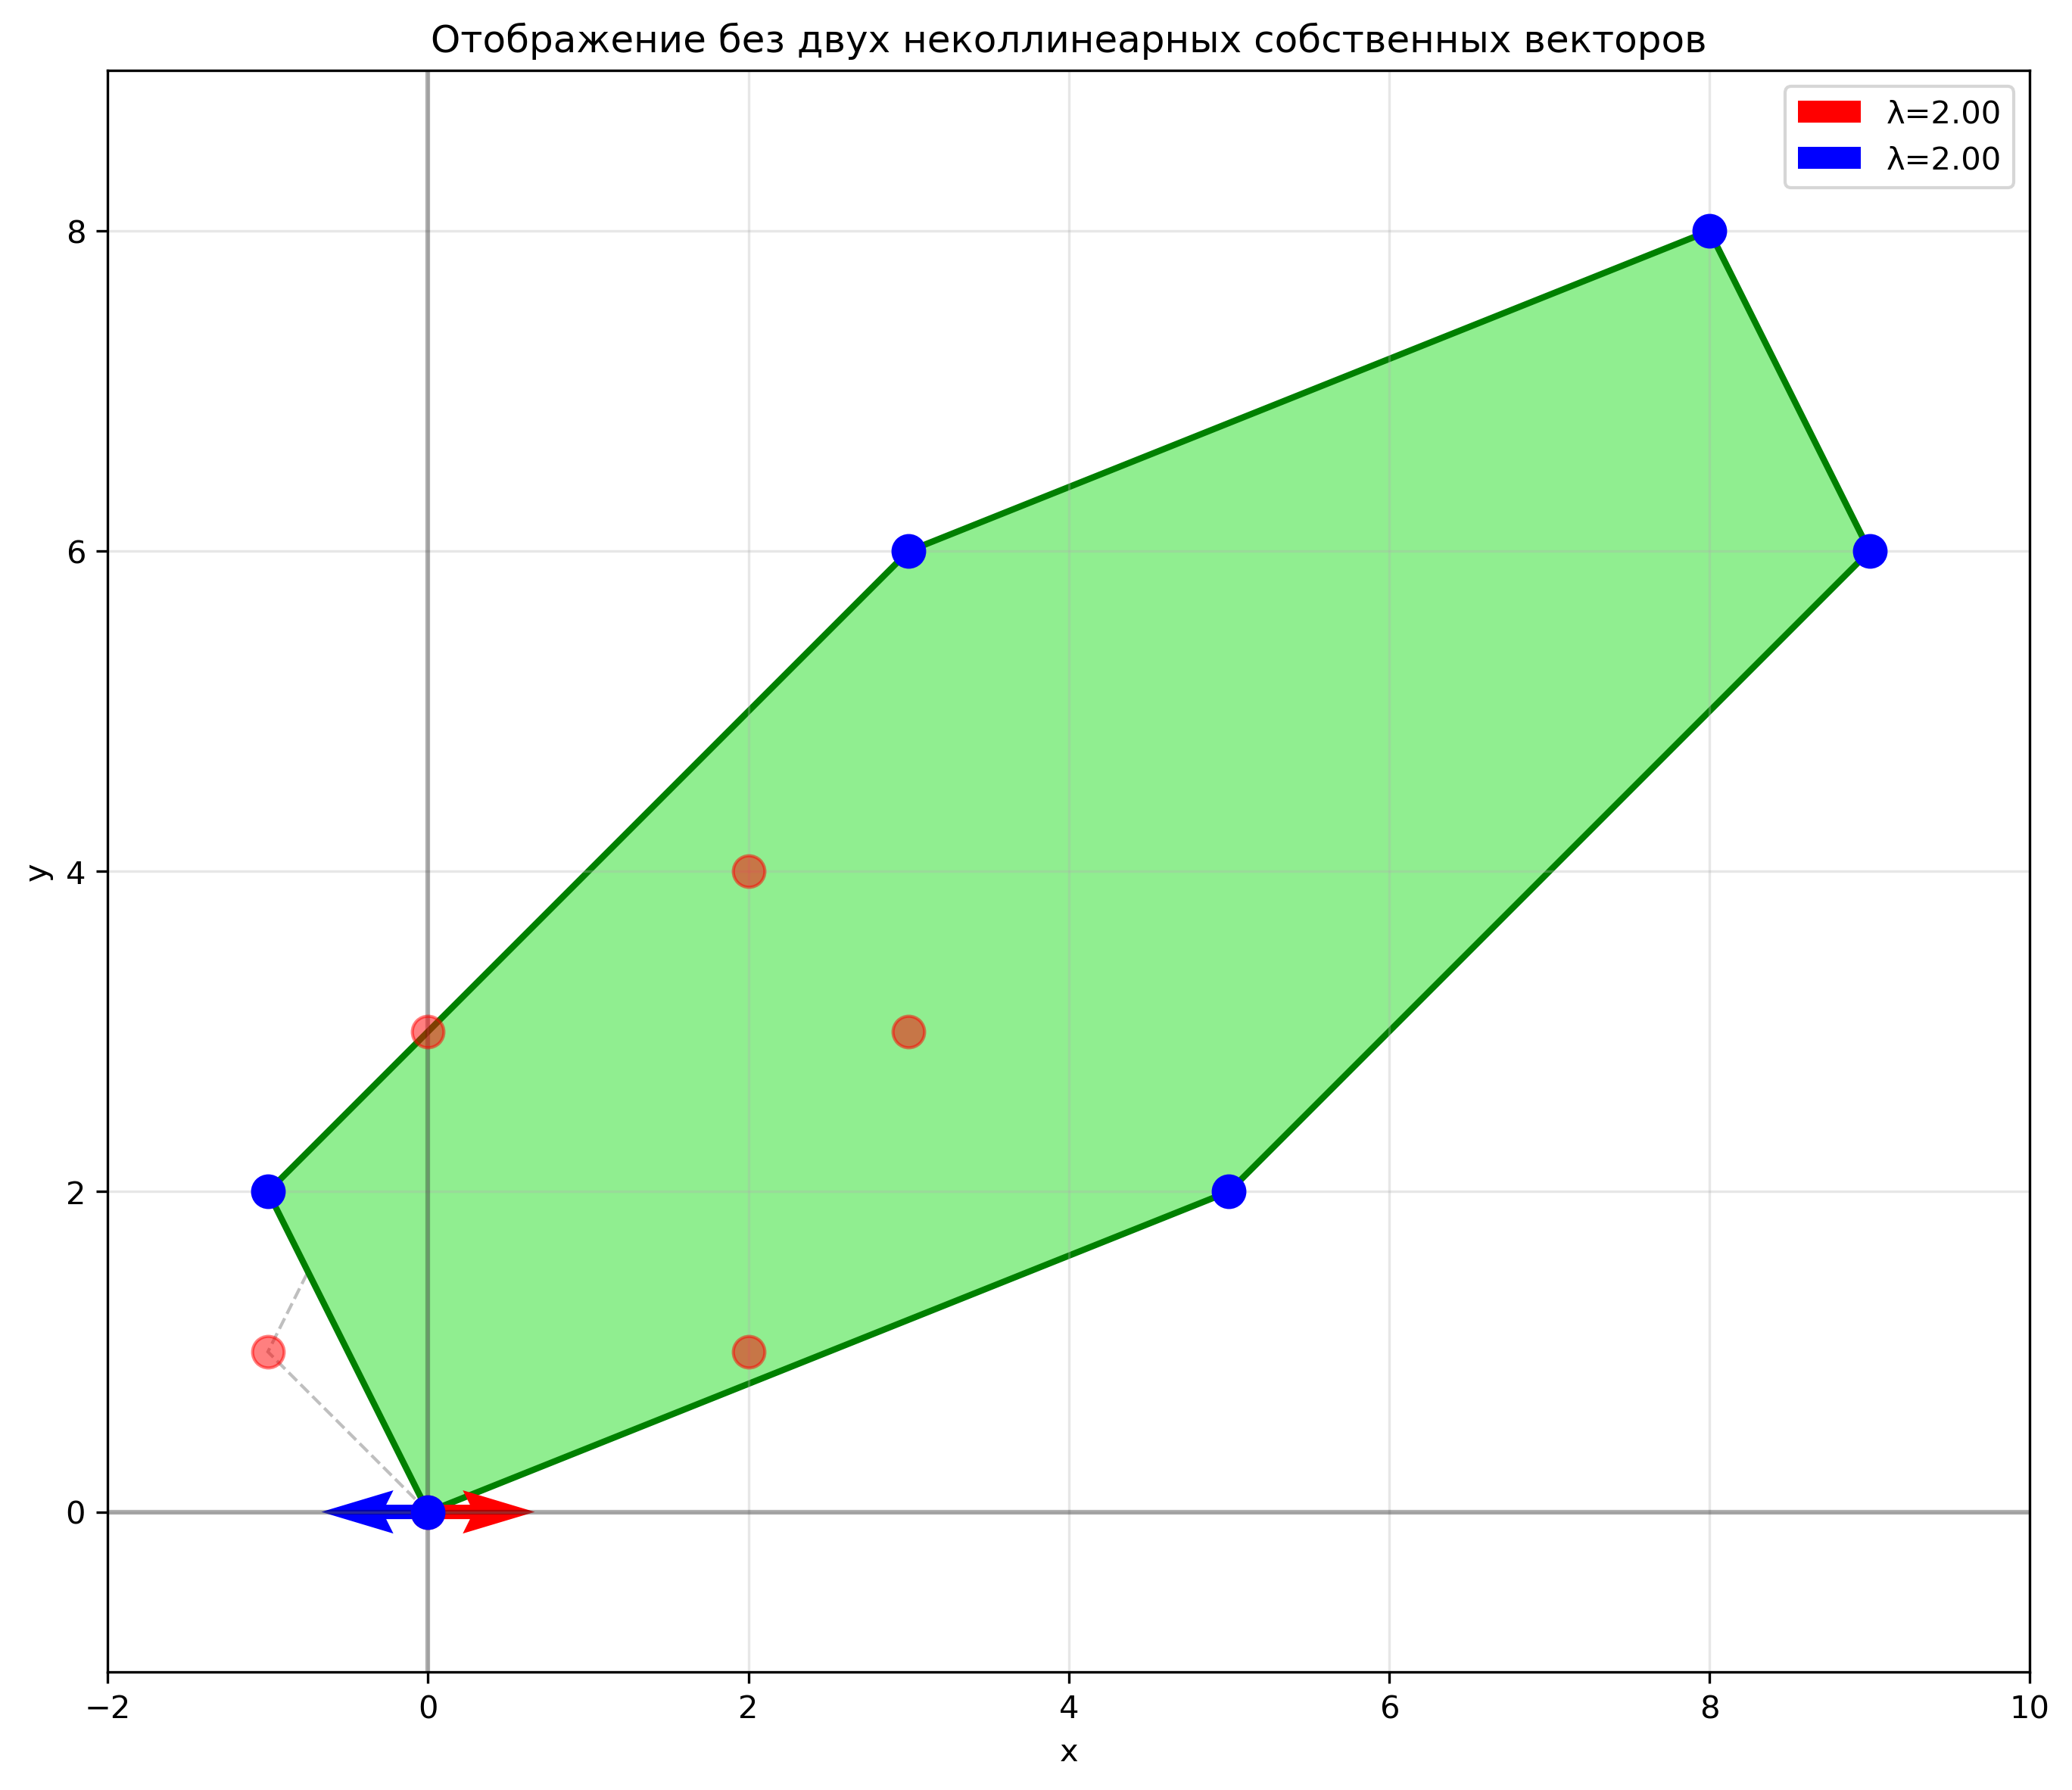
\includegraphics[width=\textwidth]{images/task1/single_eigenvector.png}
\caption{Отображение без двух неколлинеарных собственных векторов}
\label{fig:single_eigenvector}
\end{minipage}
\hfill
\begin{minipage}{0.31\textwidth}
\centering
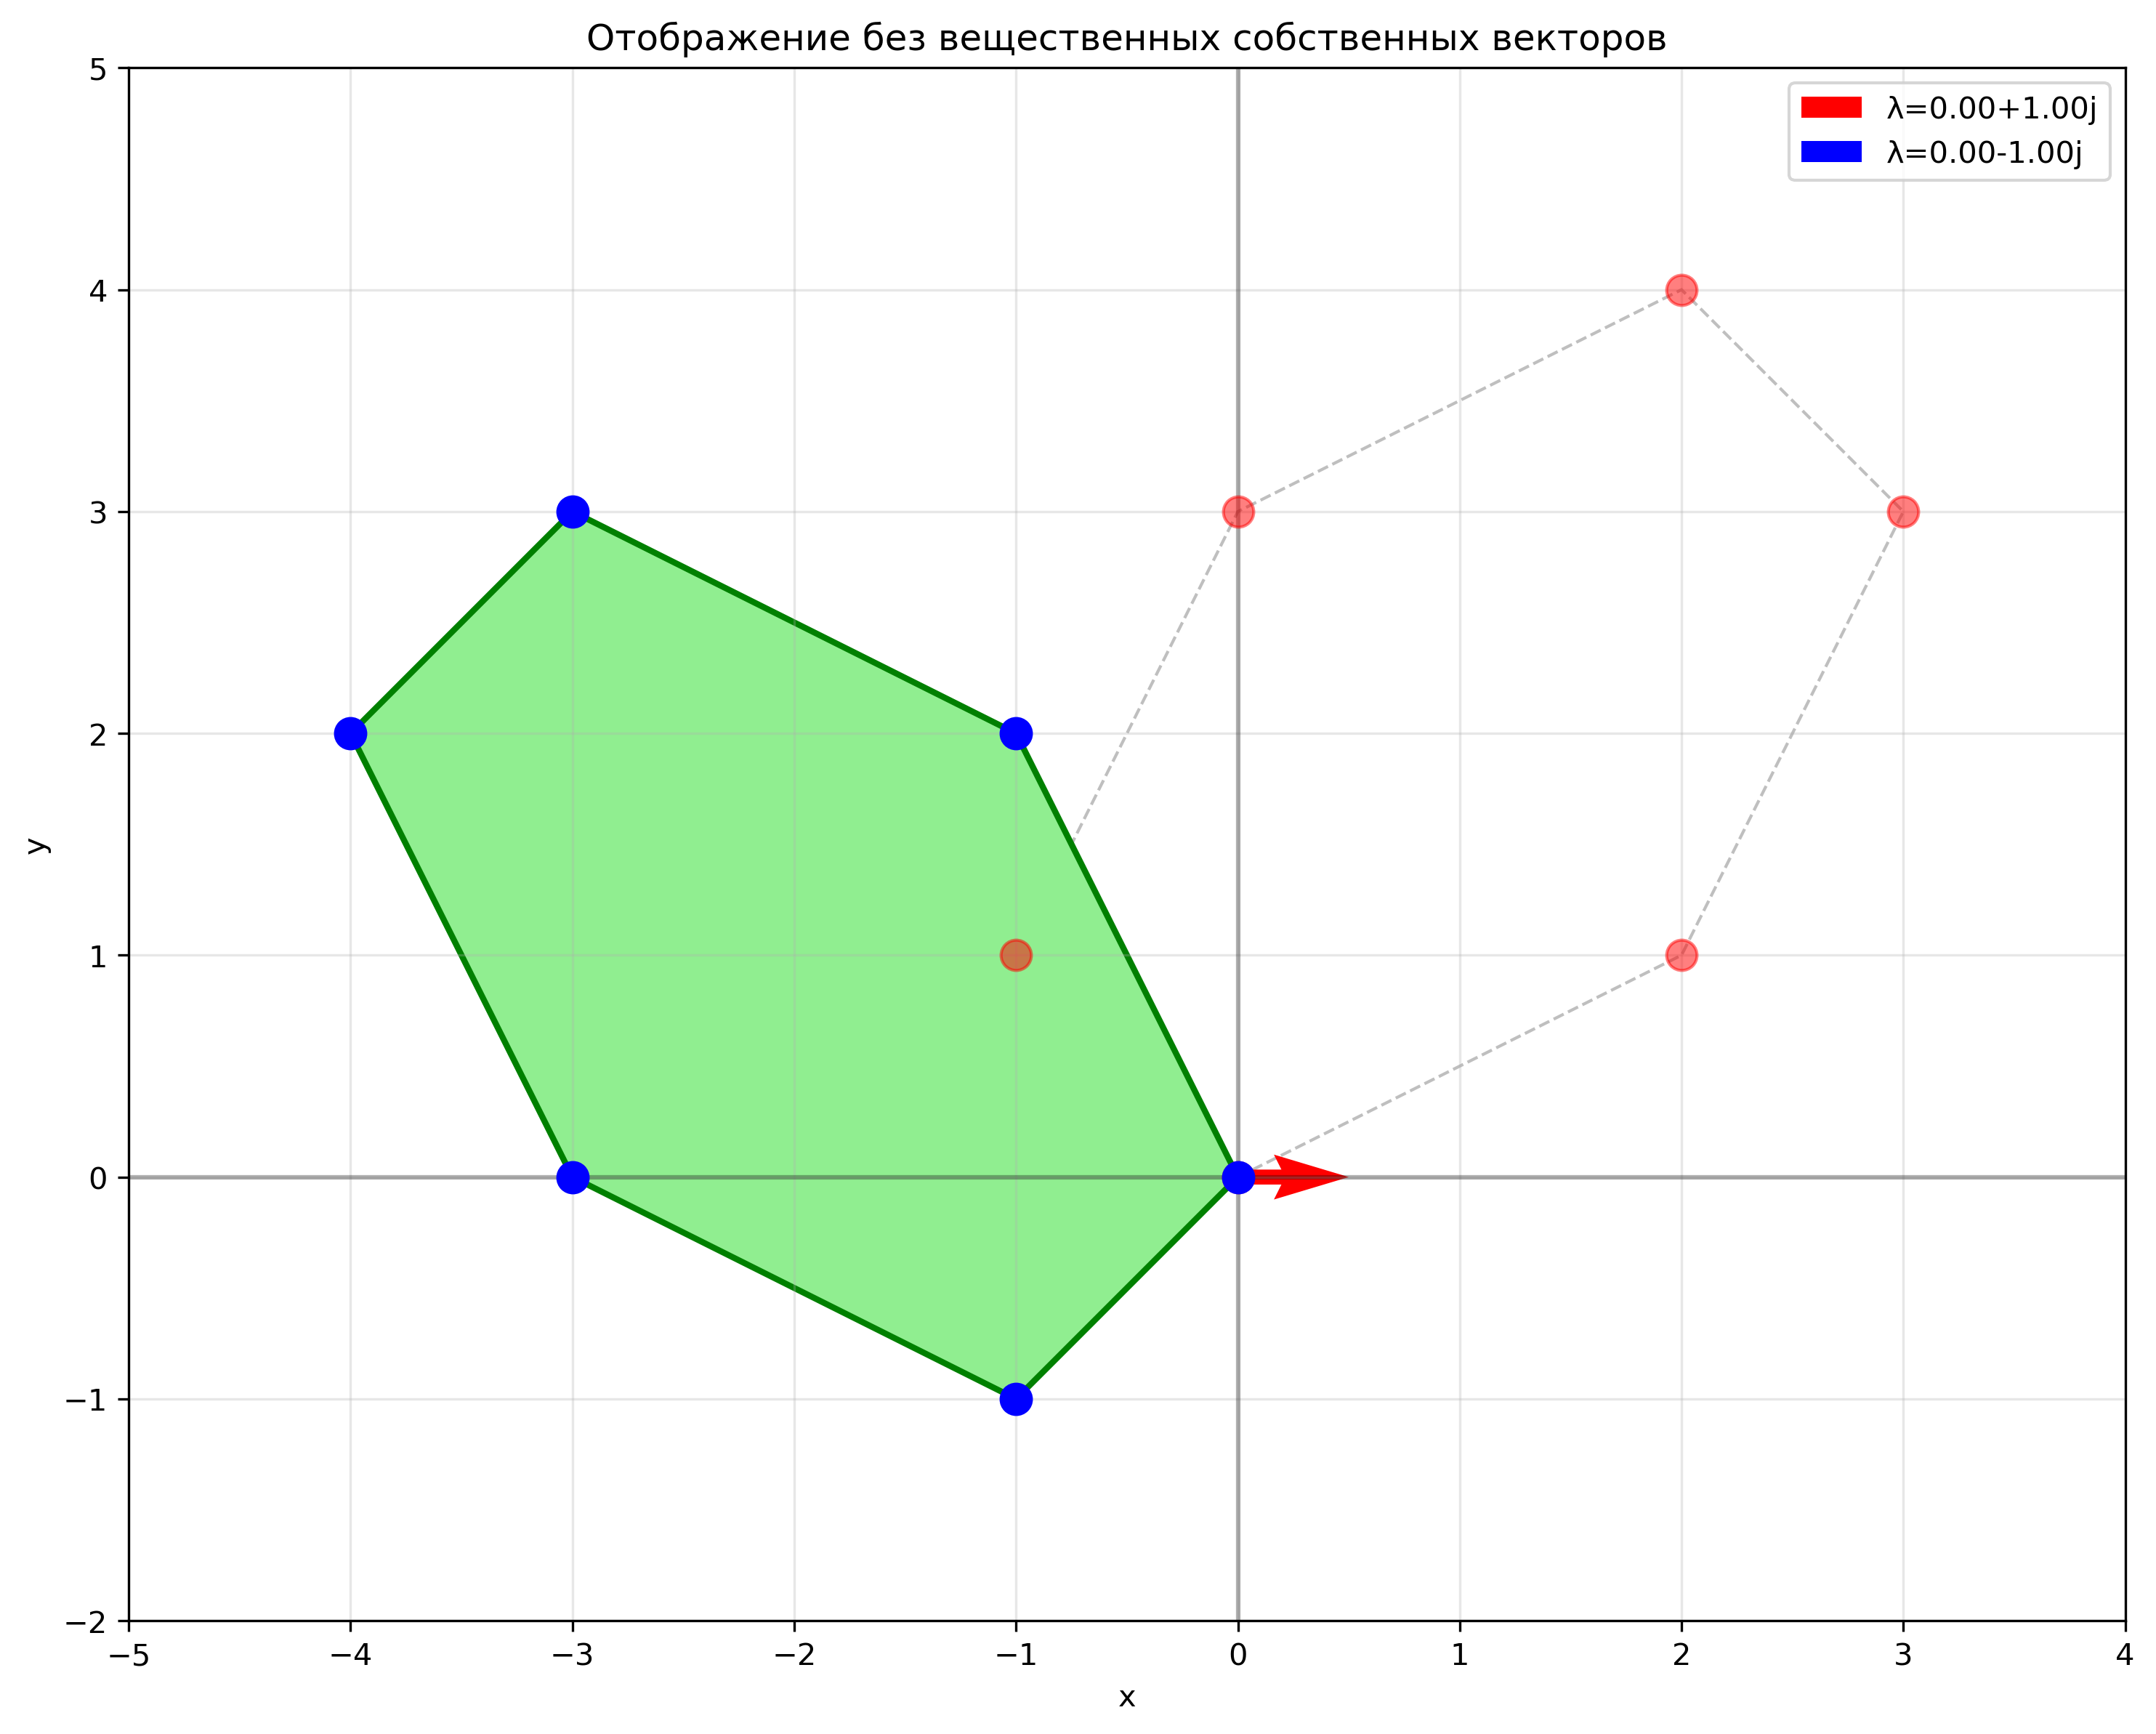
\includegraphics[width=\textwidth]{images/task1/complex_eigenvalues.png}
\caption{Отображение без вещественных собственных векторов}
\label{fig:complex_eigenvalues}
\end{minipage}
\end{figure}

\begin{figure}[h]
\centering
\begin{minipage}{0.31\textwidth}
\centering
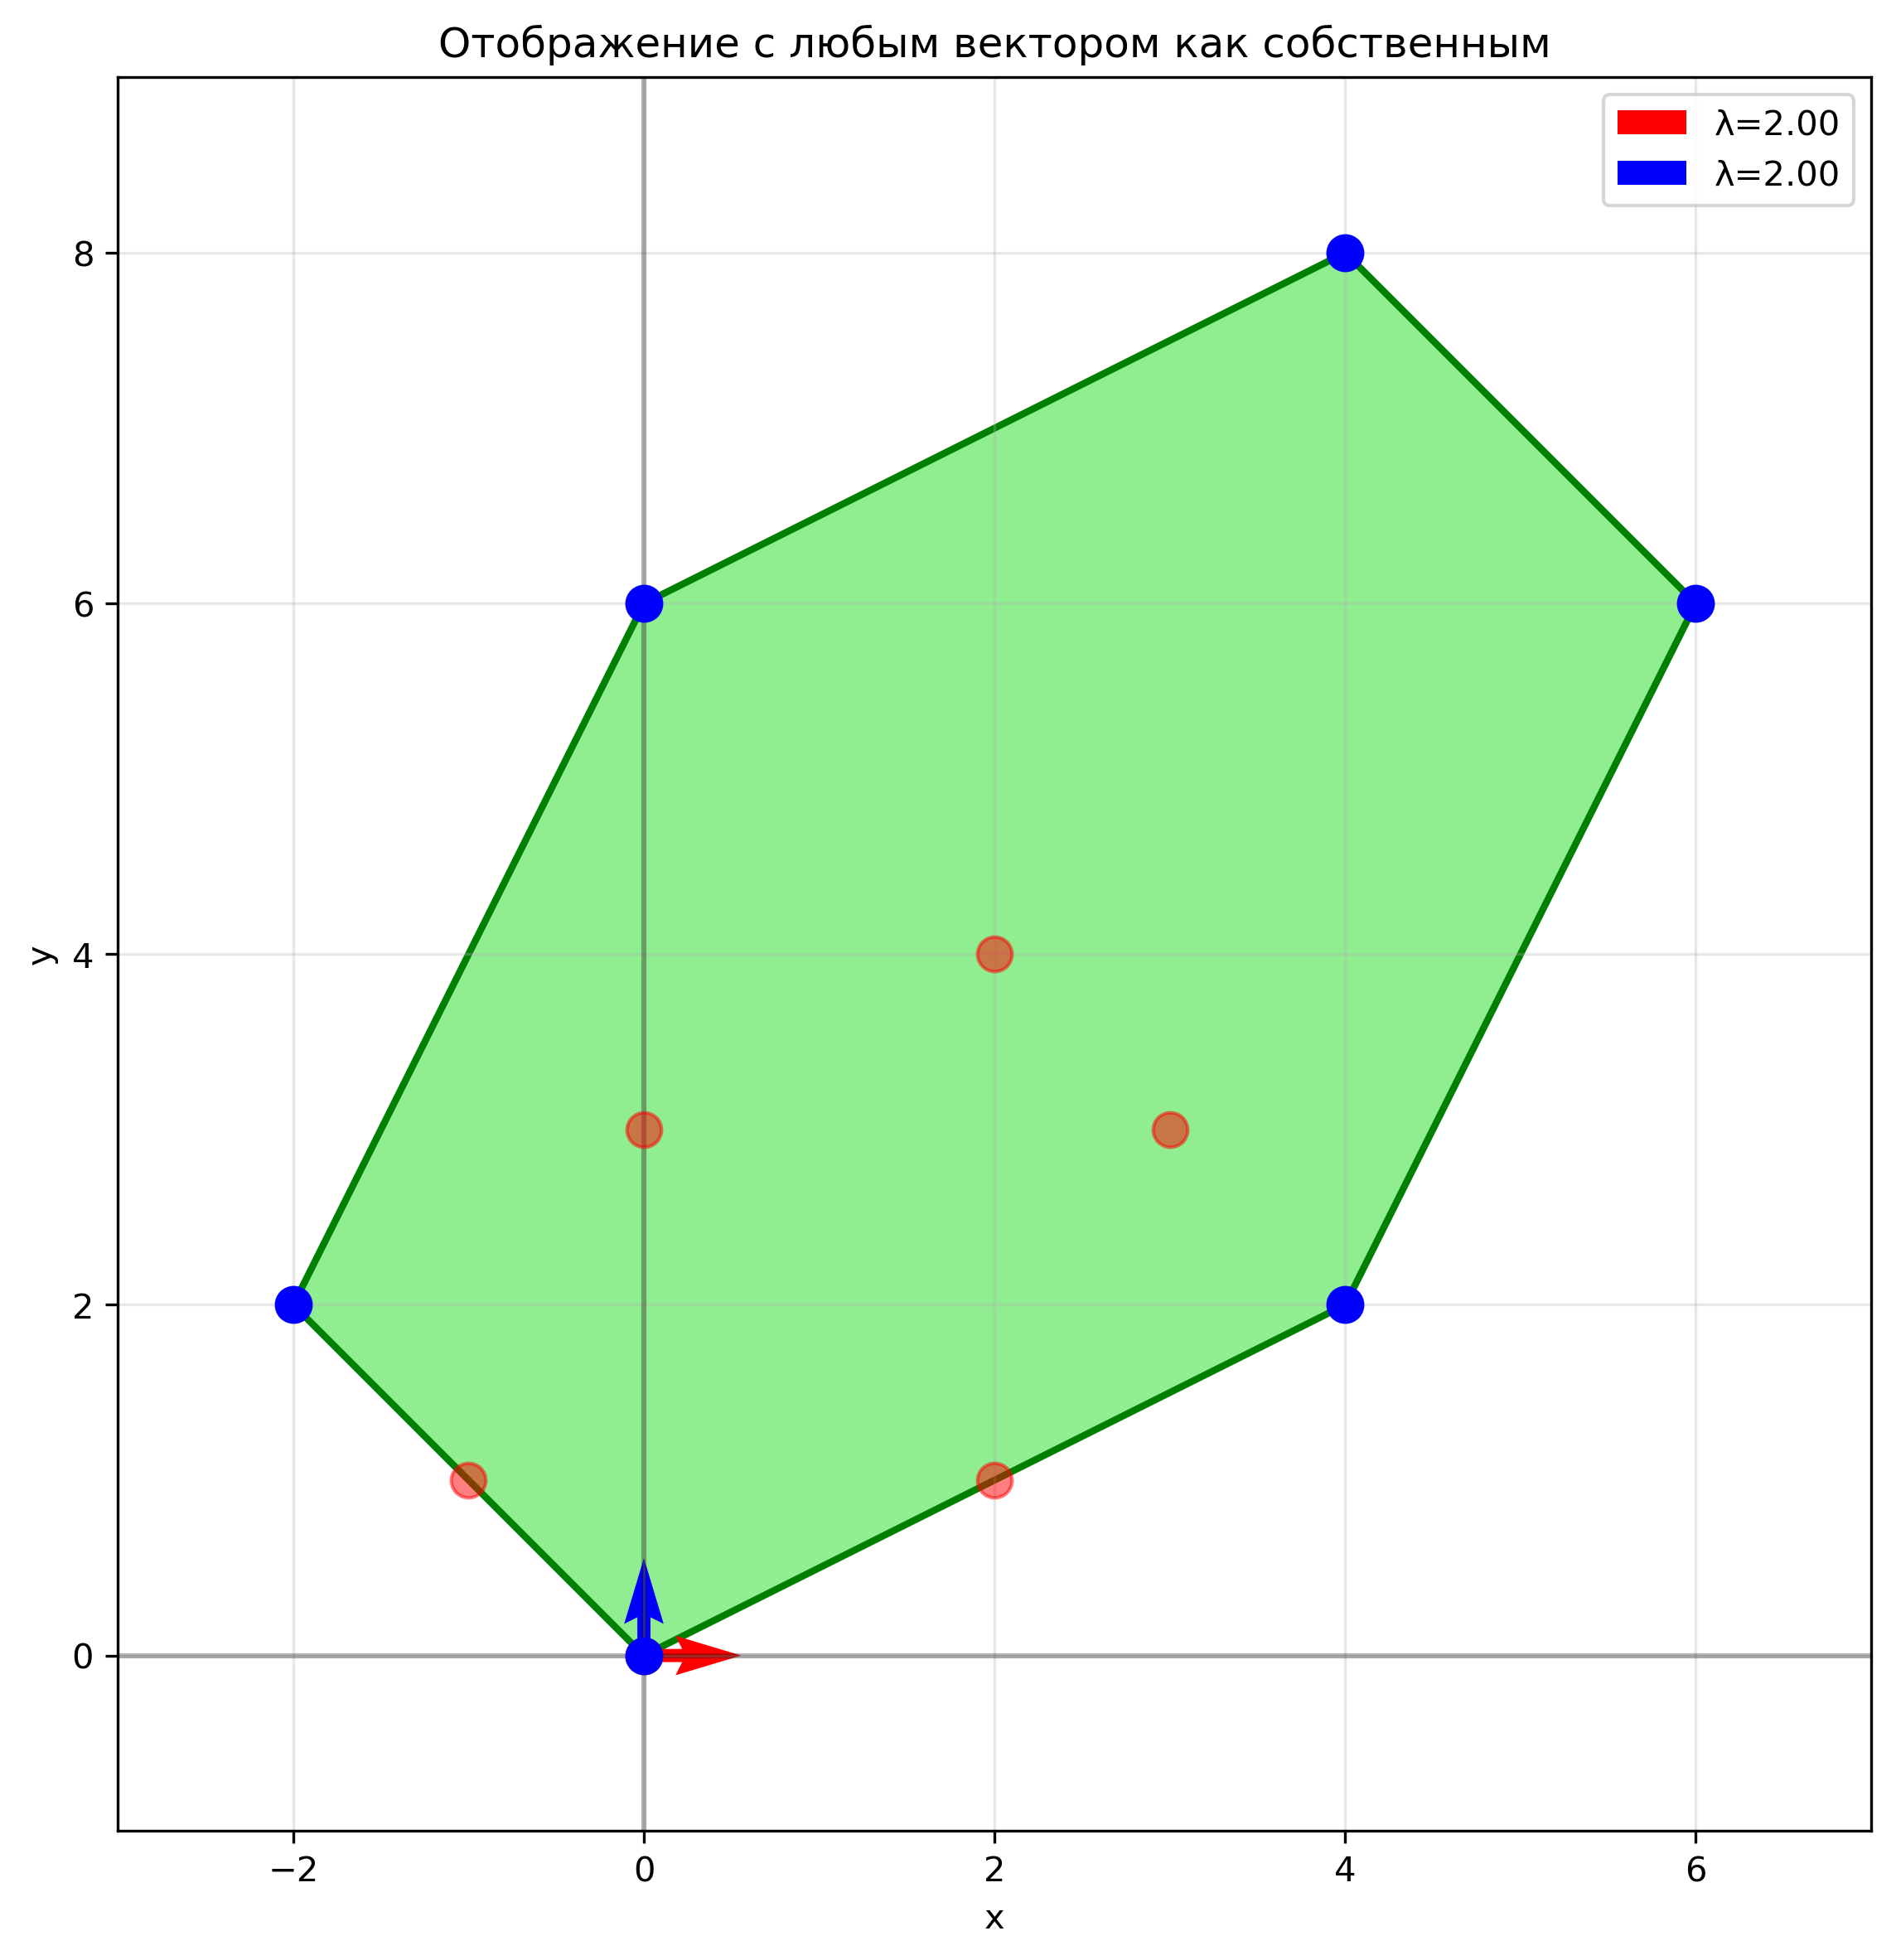
\includegraphics[width=\textwidth]{images/task1/any_vector_eigenvector.png}
\caption{Отображение с любым вектором как собственным}
\label{fig:any_vector_eigenvector}
\end{minipage}
\end{figure}

\subsection*{Пару отображений с $AB \neq BA$}

Матрицы:
\begin{equation}
A = \begin{bmatrix} 1 & 1 \\ 0 & 1 \end{bmatrix}, \quad
B = \begin{bmatrix} 1 & 0 \\ 1 & 1 \end{bmatrix}
\end{equation}

Произведения:
\begin{equation}
AB = \begin{bmatrix} 2 & 1 \\ 1 & 1 \end{bmatrix}, \quad
BA = \begin{bmatrix} 1 & 1 \\ 1 & 2 \end{bmatrix}
\end{equation}

Действительно, $AB \neq BA$.

\begin{figure}[h]
\centering
\begin{minipage}{0.23\textwidth}
\centering
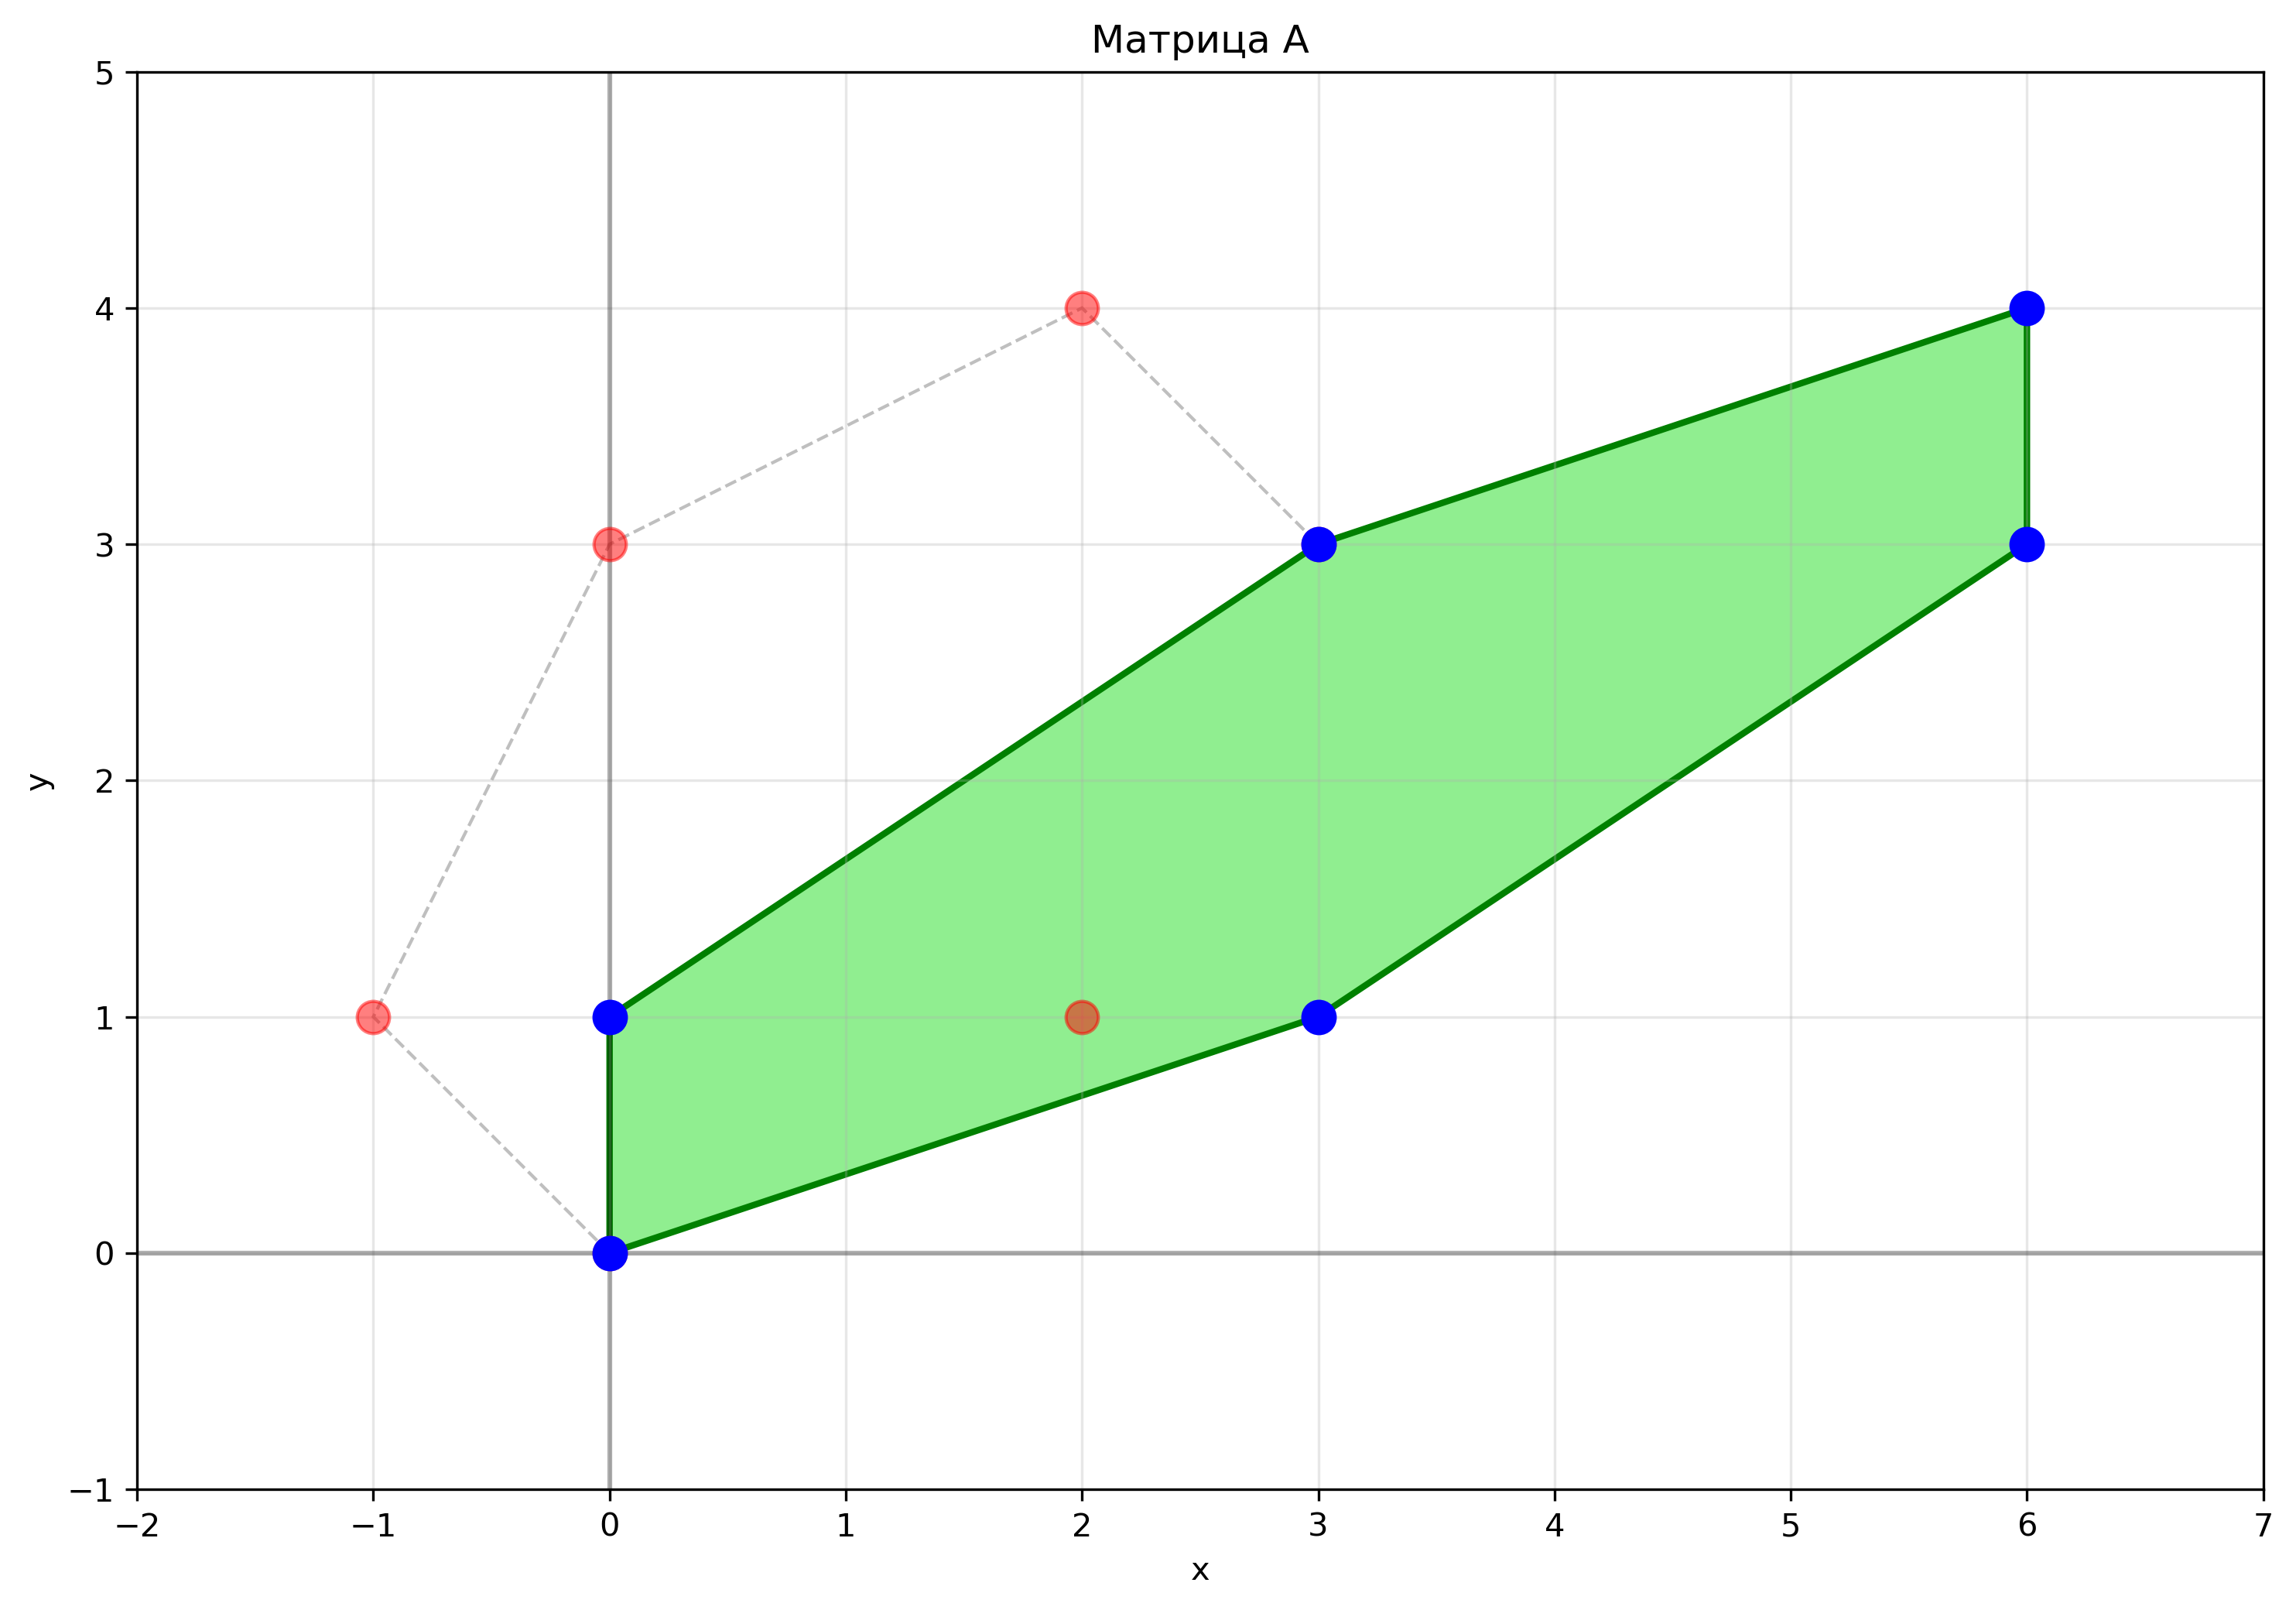
\includegraphics[width=\textwidth]{images/task1/matrix_A.png}
\caption{Матрица $A$}
\label{fig:matrix_A}
\end{minipage}
\hfill
\begin{minipage}{0.23\textwidth}
\centering
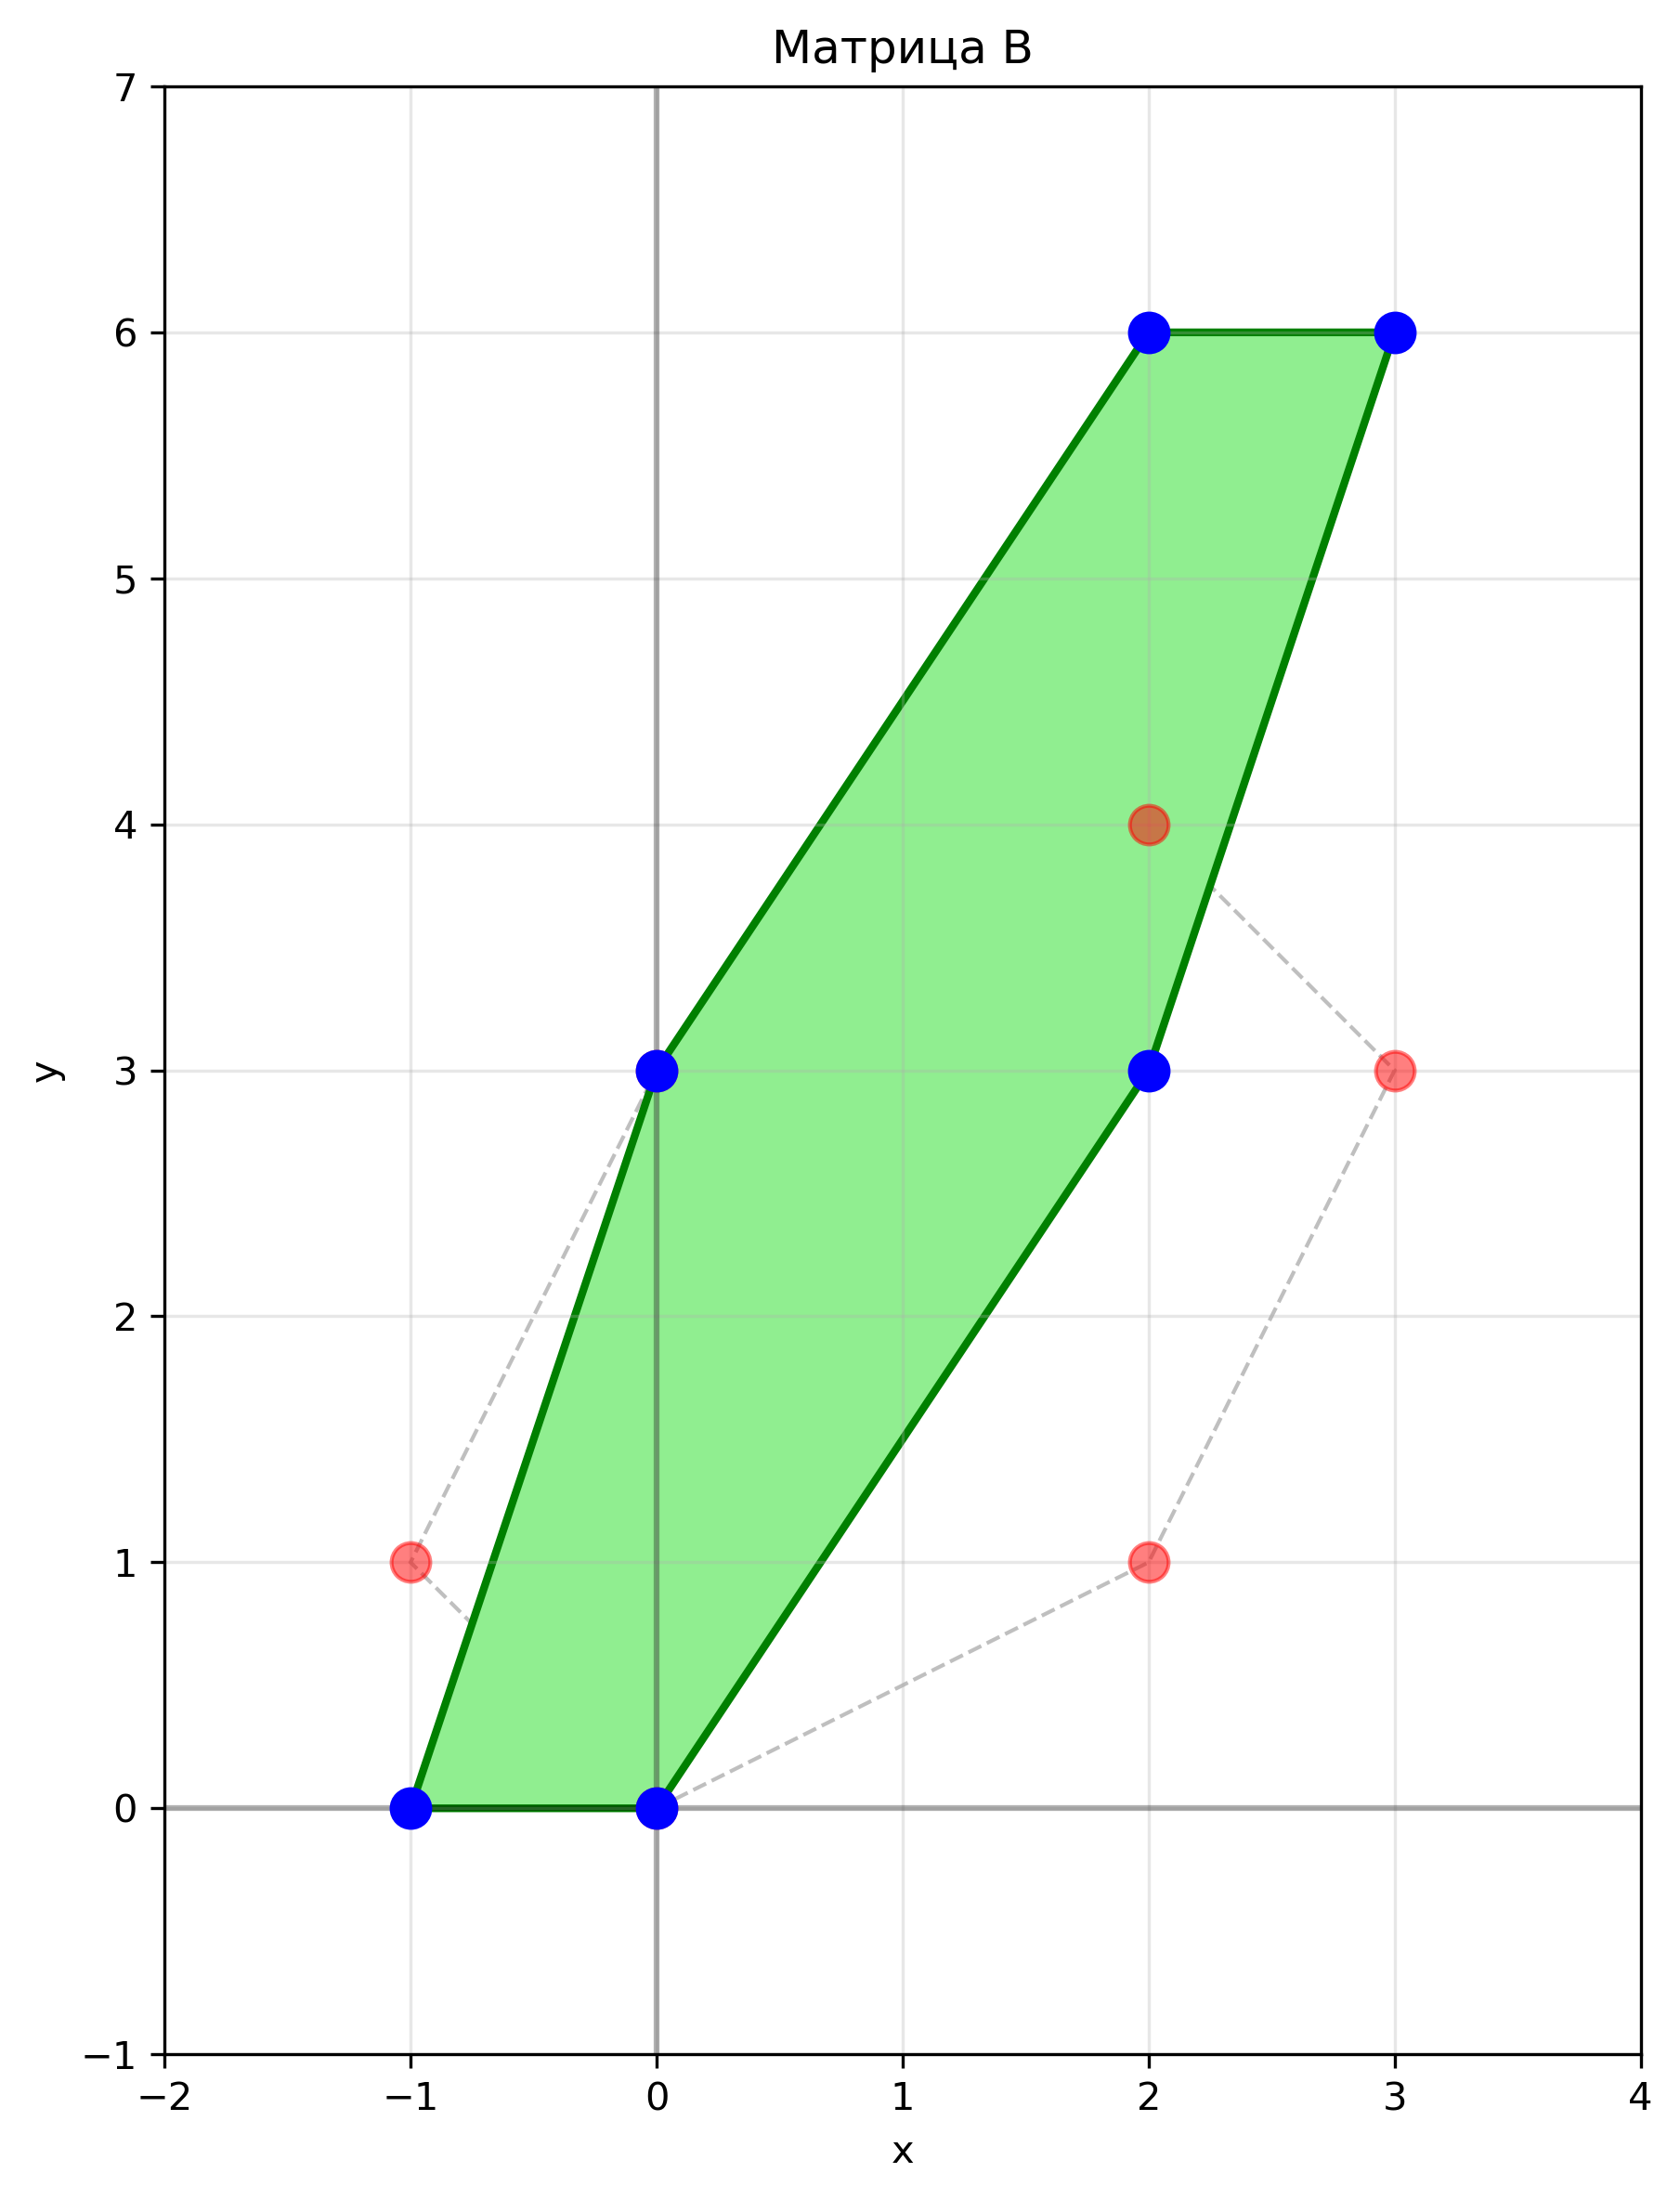
\includegraphics[width=\textwidth]{images/task1/matrix_B.png}
\caption{Матрица $B$}
\label{fig:matrix_B}
\end{minipage}
\hfill
\begin{minipage}{0.23\textwidth}
\centering
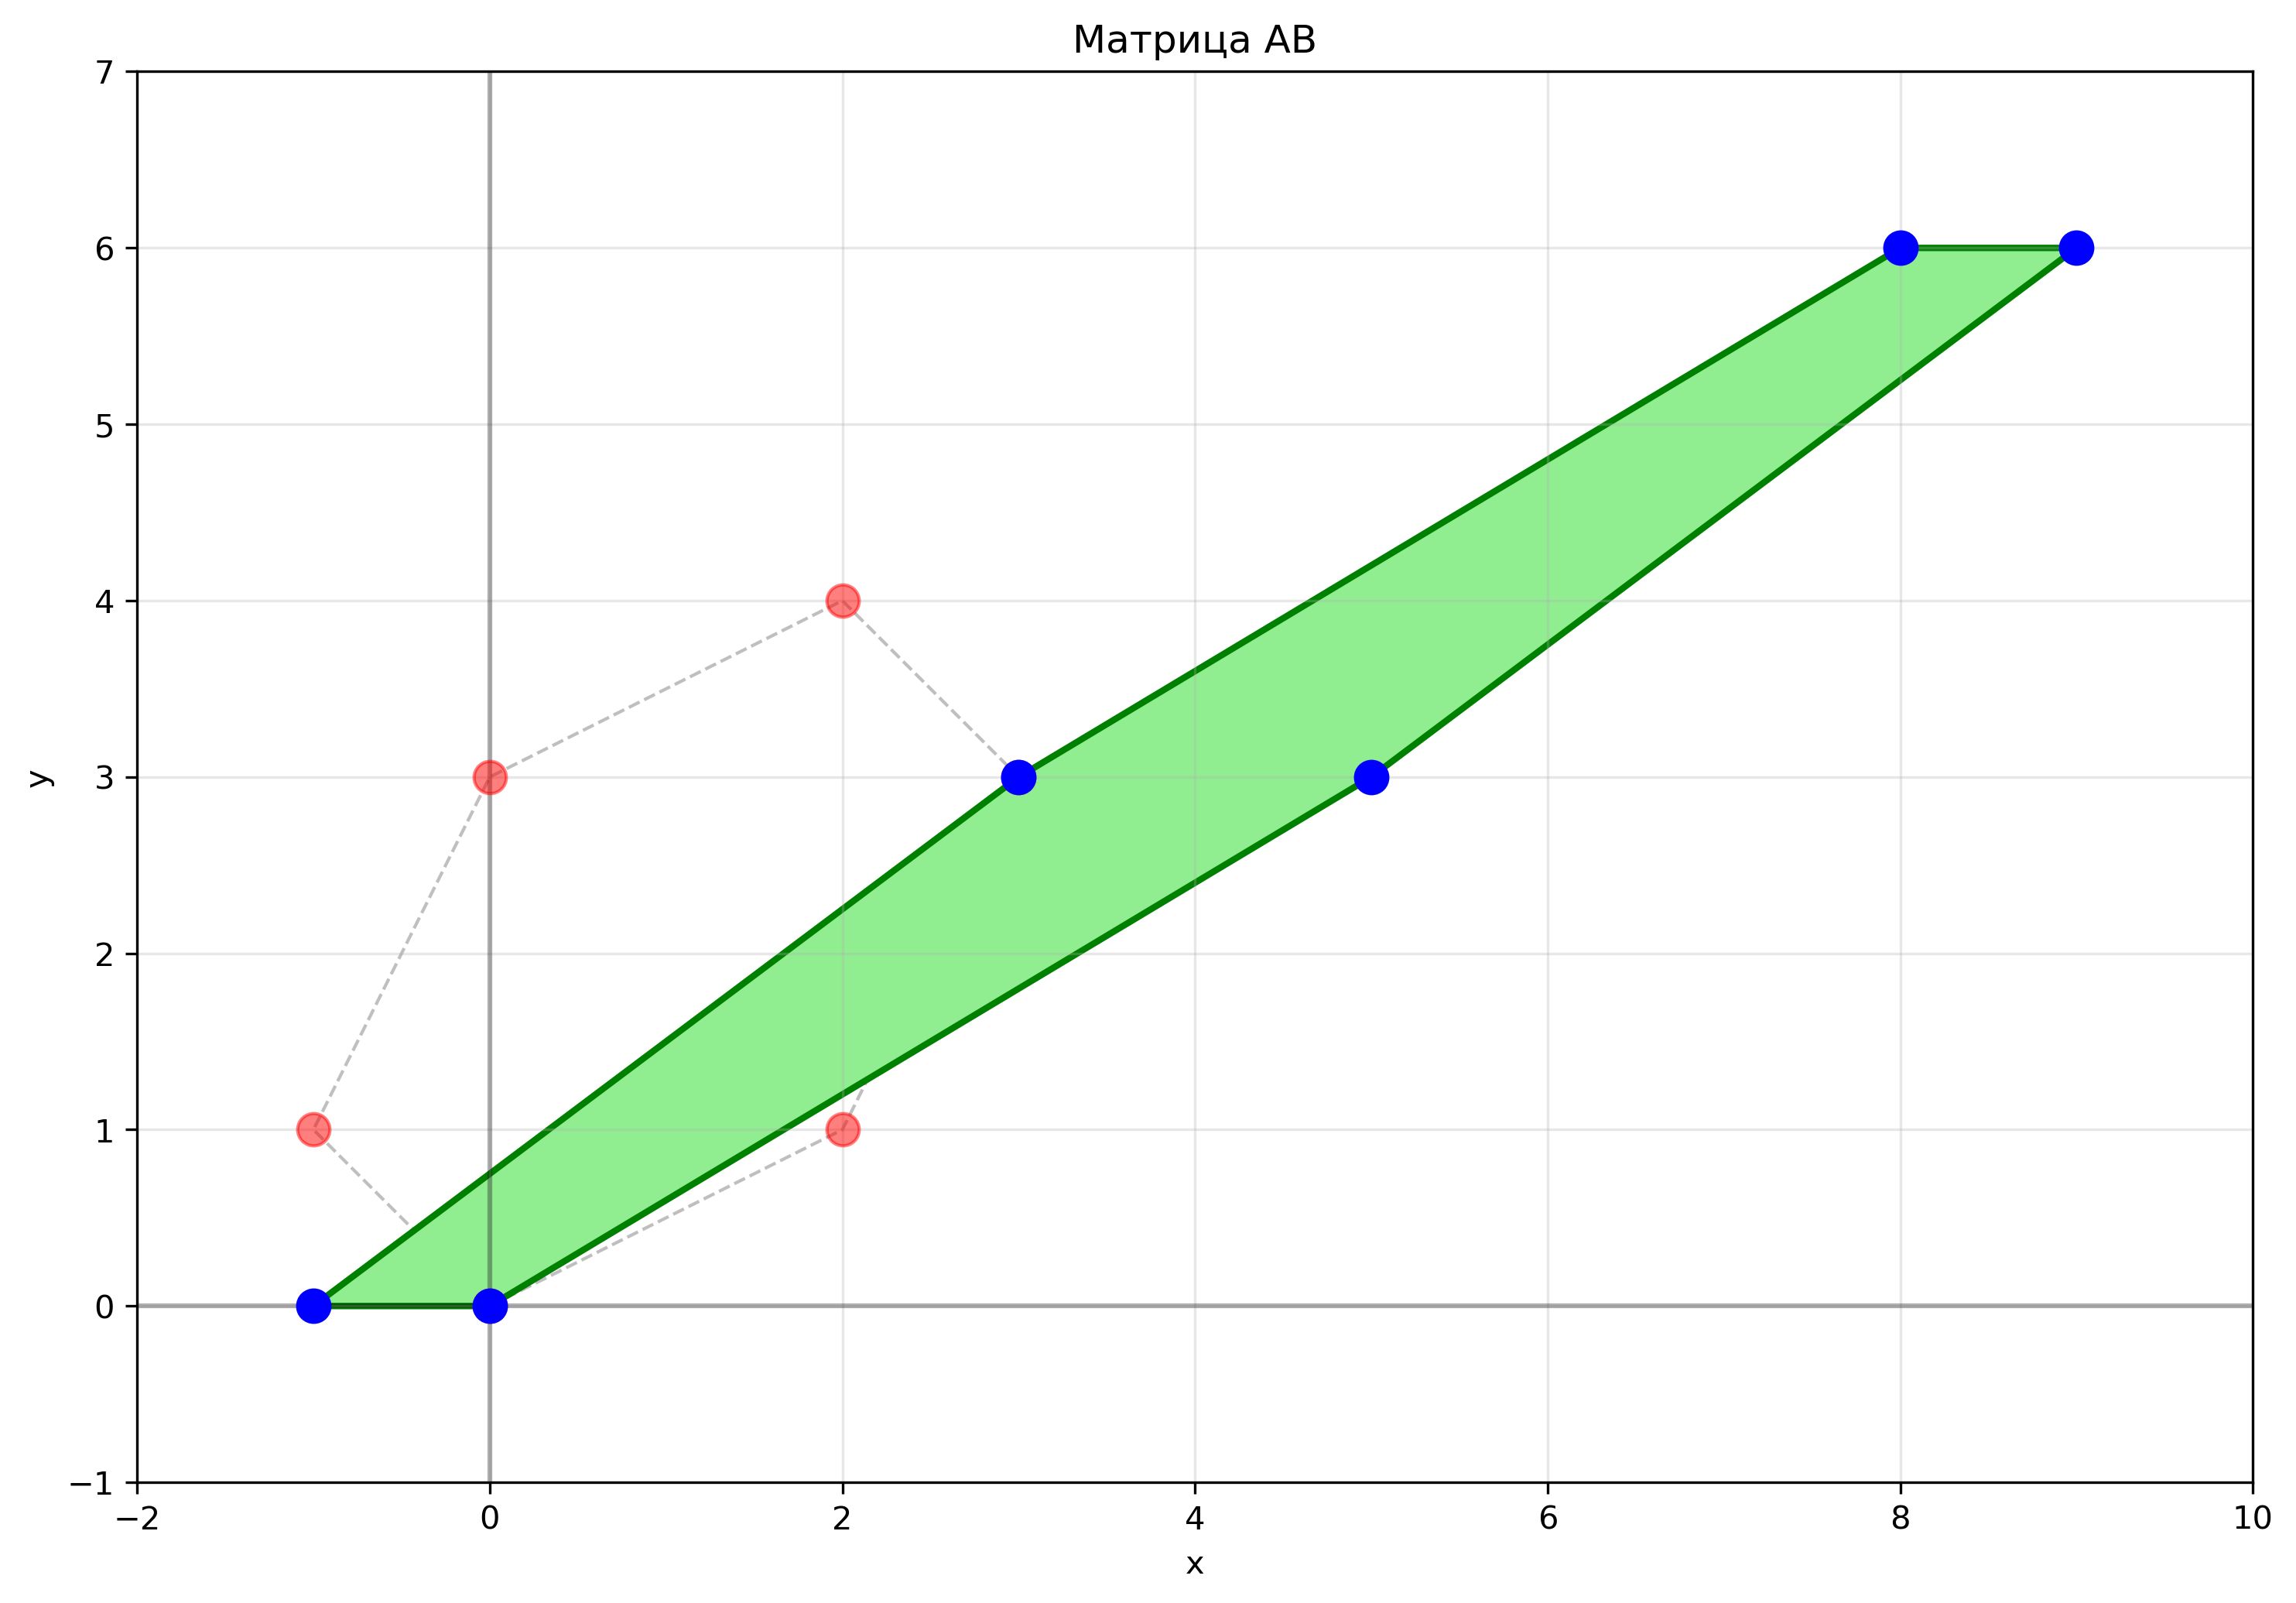
\includegraphics[width=\textwidth]{images/task1/matrix_AB.png}
\caption{Матрица $AB$}
\label{fig:matrix_AB}
\end{minipage}
\hfill
\begin{minipage}{0.23\textwidth}
\centering
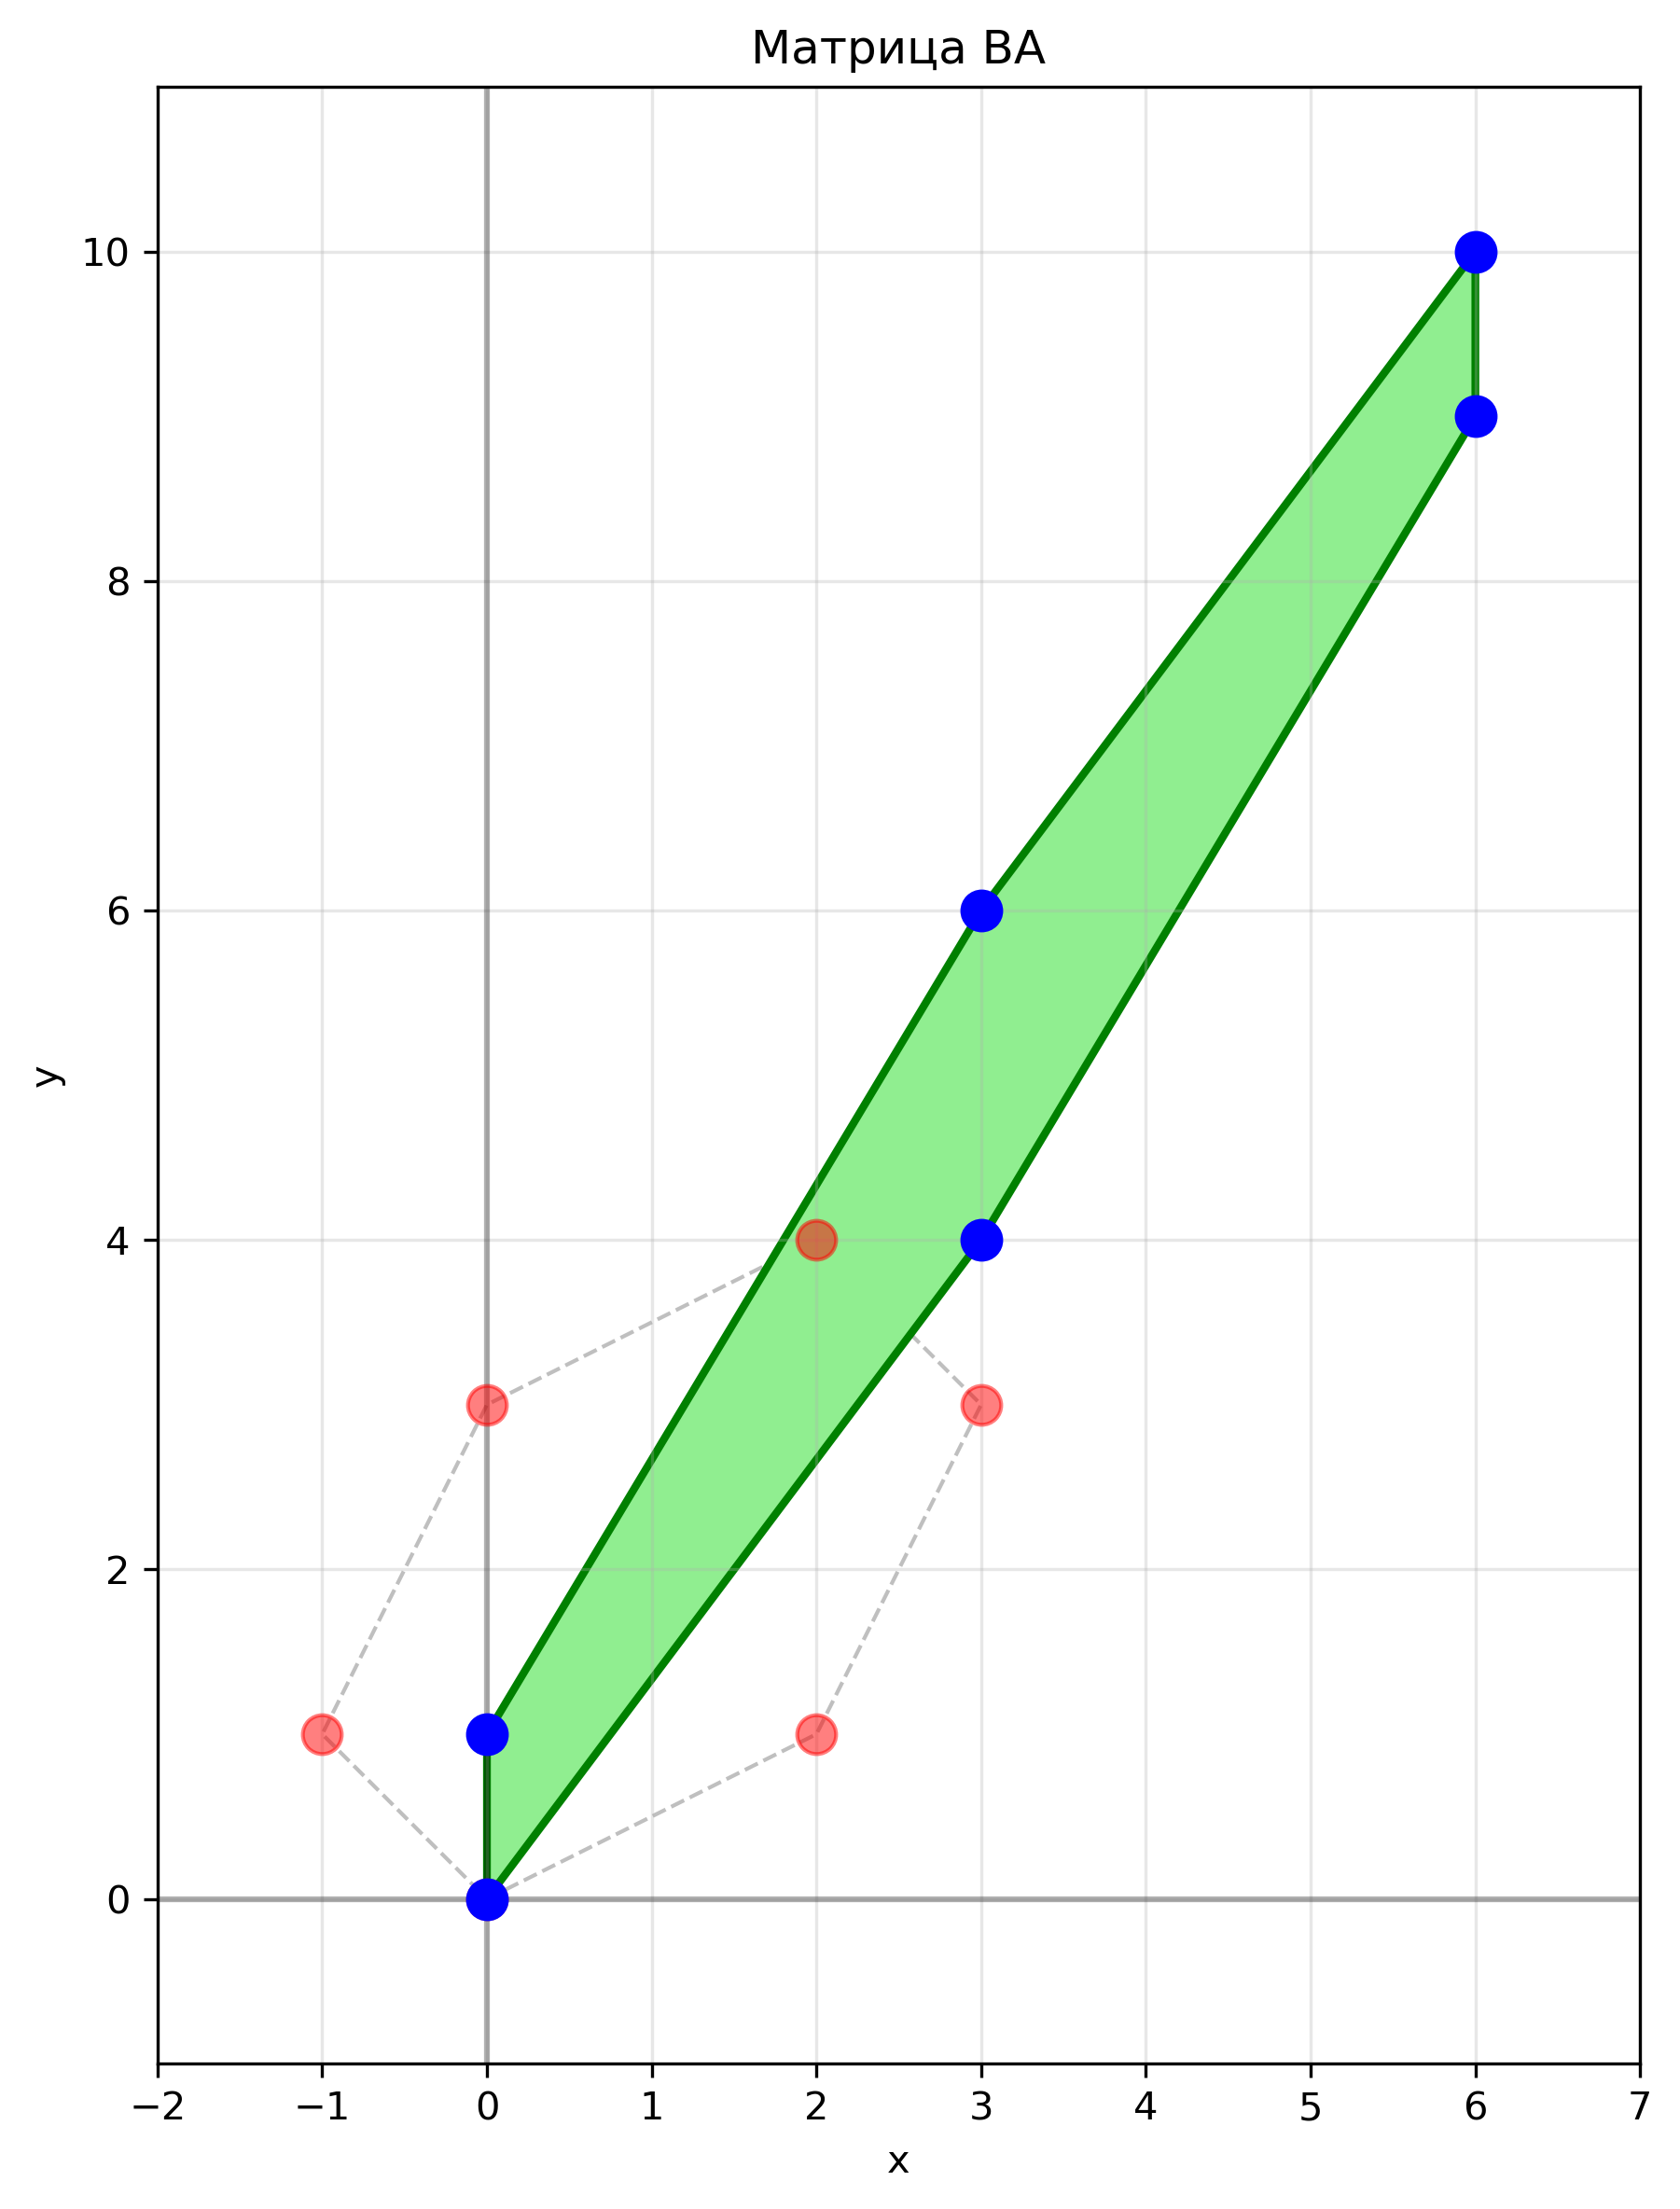
\includegraphics[width=\textwidth]{images/task1/matrix_BA.png}
\caption{Матрица $BA$}
\label{fig:matrix_BA}
\end{minipage}
\end{figure}

\subsection*{Пару отображений с $AB = BA$}

Матрицы:
\begin{equation}
C = \begin{bmatrix} 2 & 0 \\ 0 & 3 \end{bmatrix}, \quad
D = \begin{bmatrix} 1 & 0 \\ 0 & 4 \end{bmatrix}
\end{equation}

Произведения:
\begin{equation}
CD = \begin{bmatrix} 2 & 0 \\ 0 & 12 \end{bmatrix}, \quad
DC = \begin{bmatrix} 2 & 0 \\ 0 & 12 \end{bmatrix}
\end{equation}

Действительно, $CD = DC$.

\begin{figure}[h]
\centering
\begin{minipage}{0.23\textwidth}
\centering
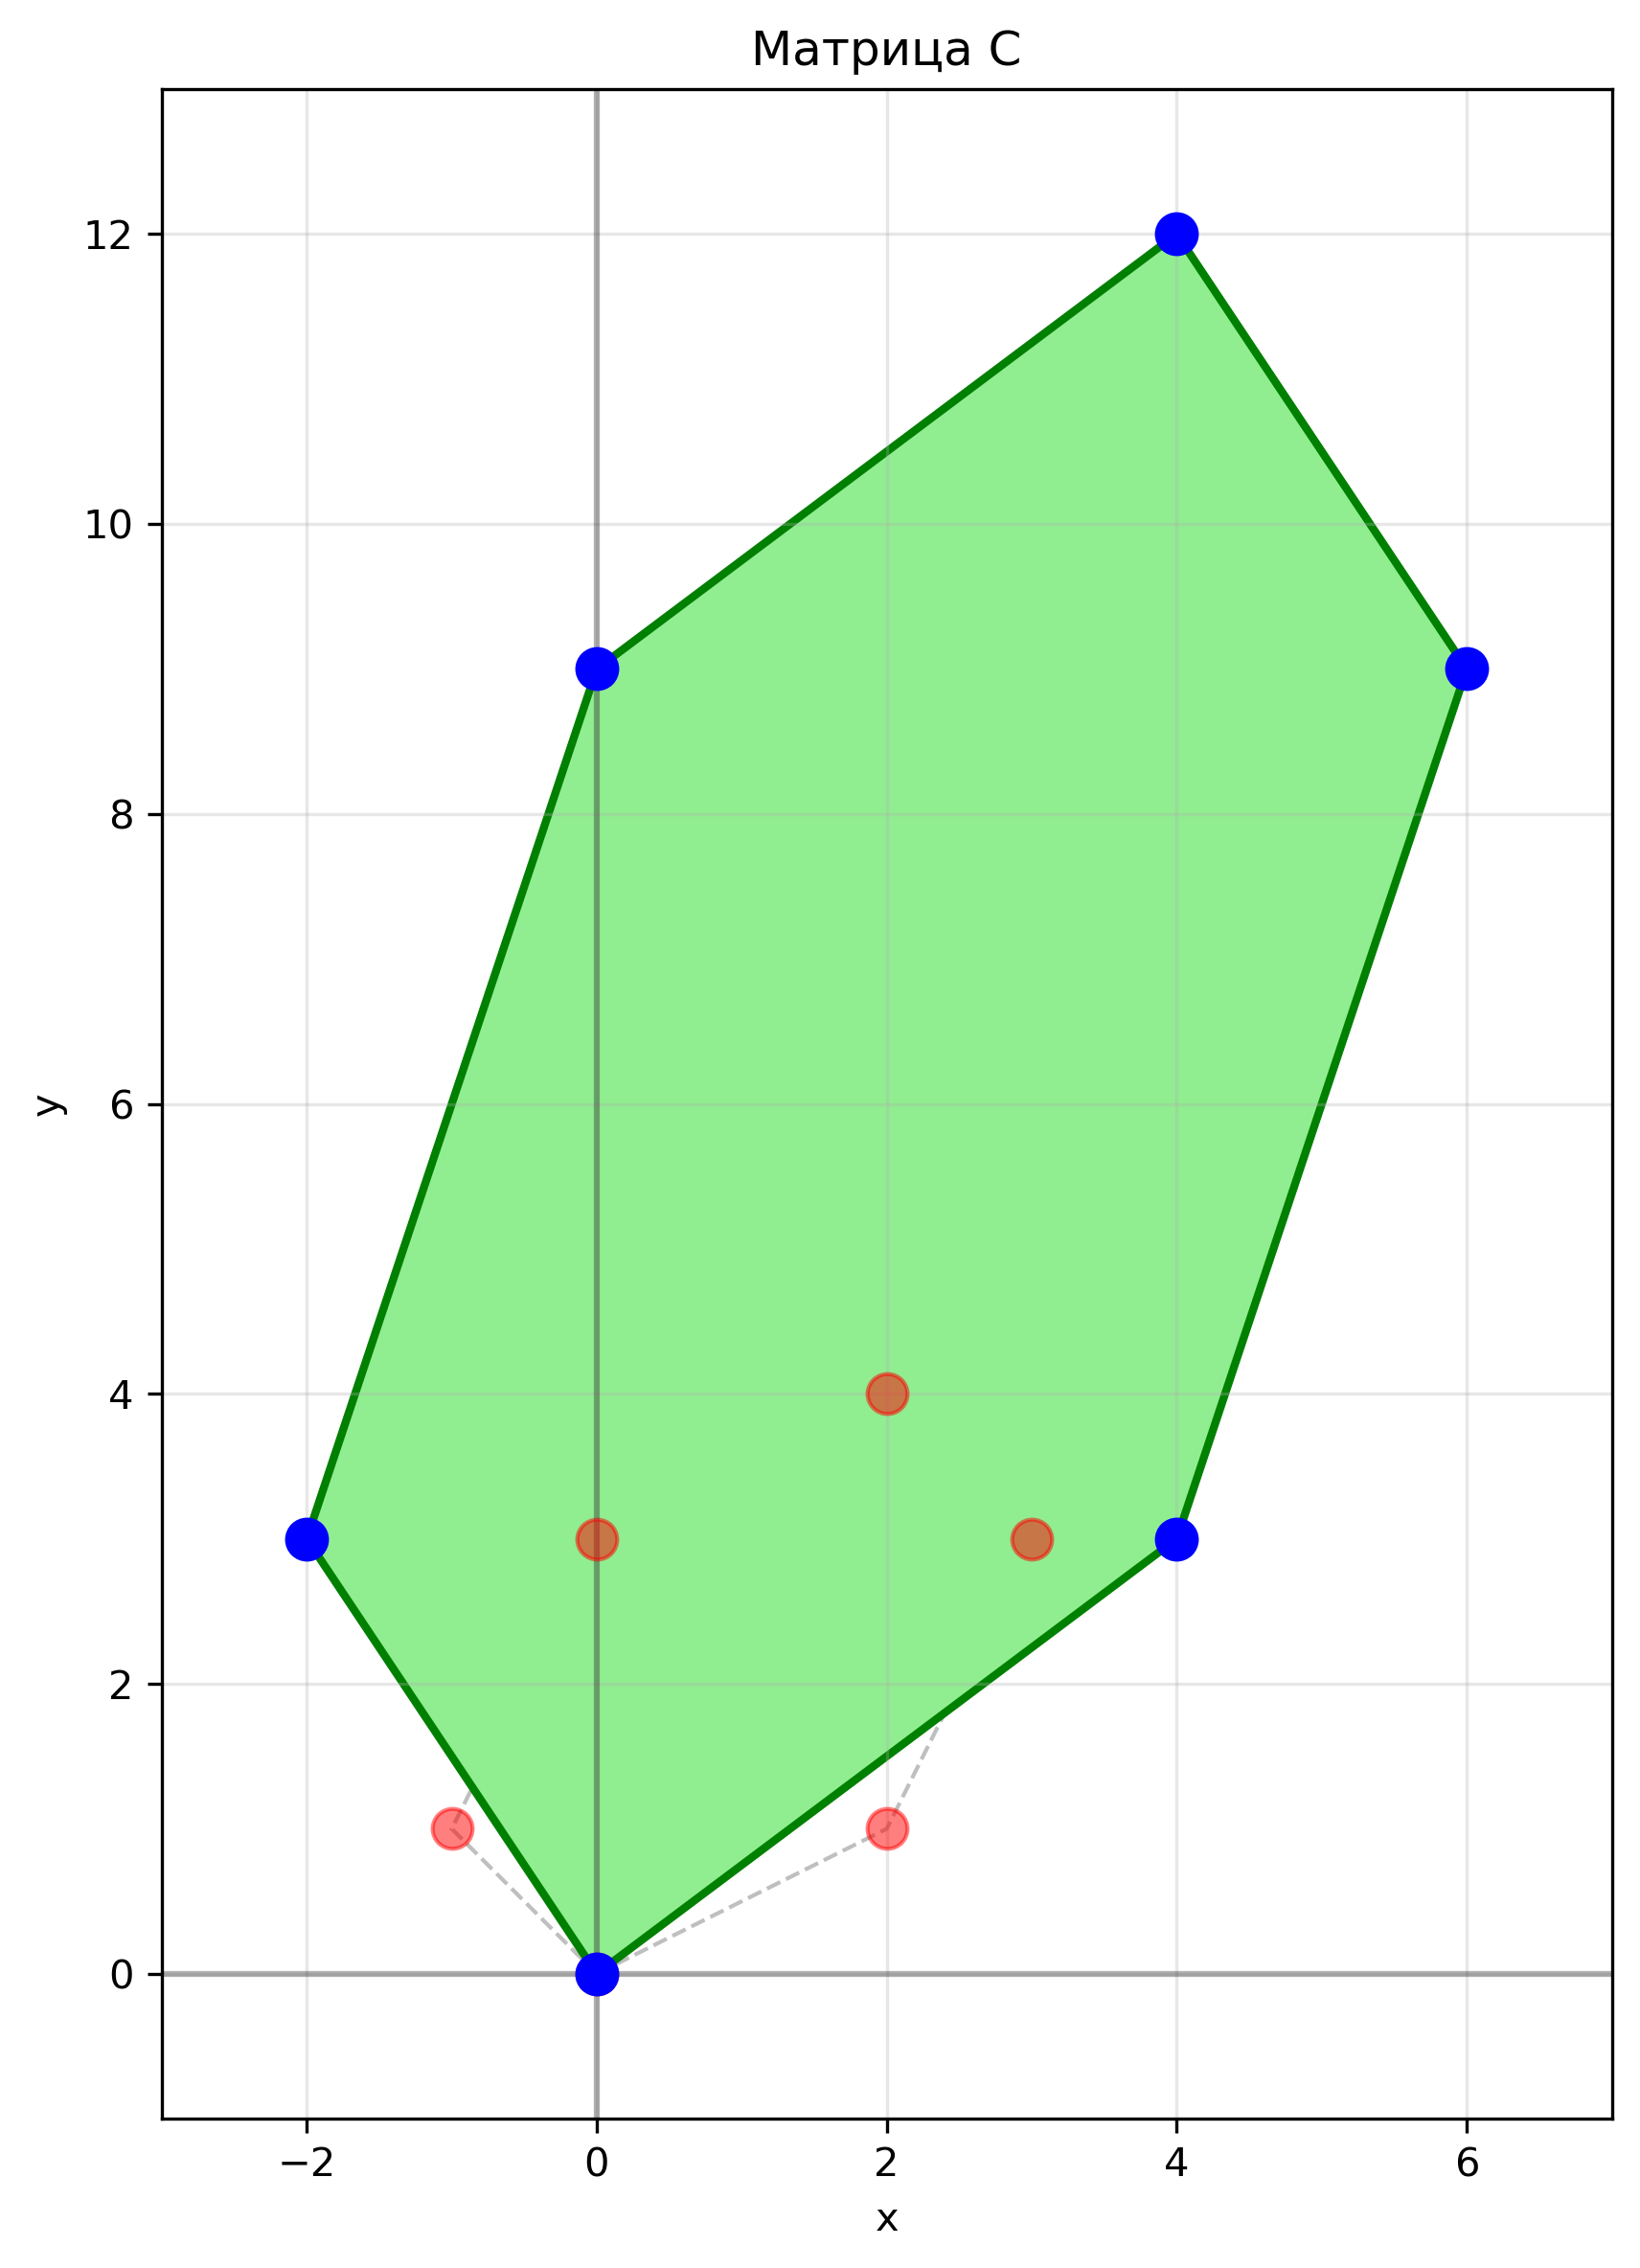
\includegraphics[width=\textwidth]{images/task1/matrix_C.png}
\caption{Матрица $C$}
\label{fig:matrix_C}
\end{minipage}
\hfill
\begin{minipage}{0.23\textwidth}
\centering
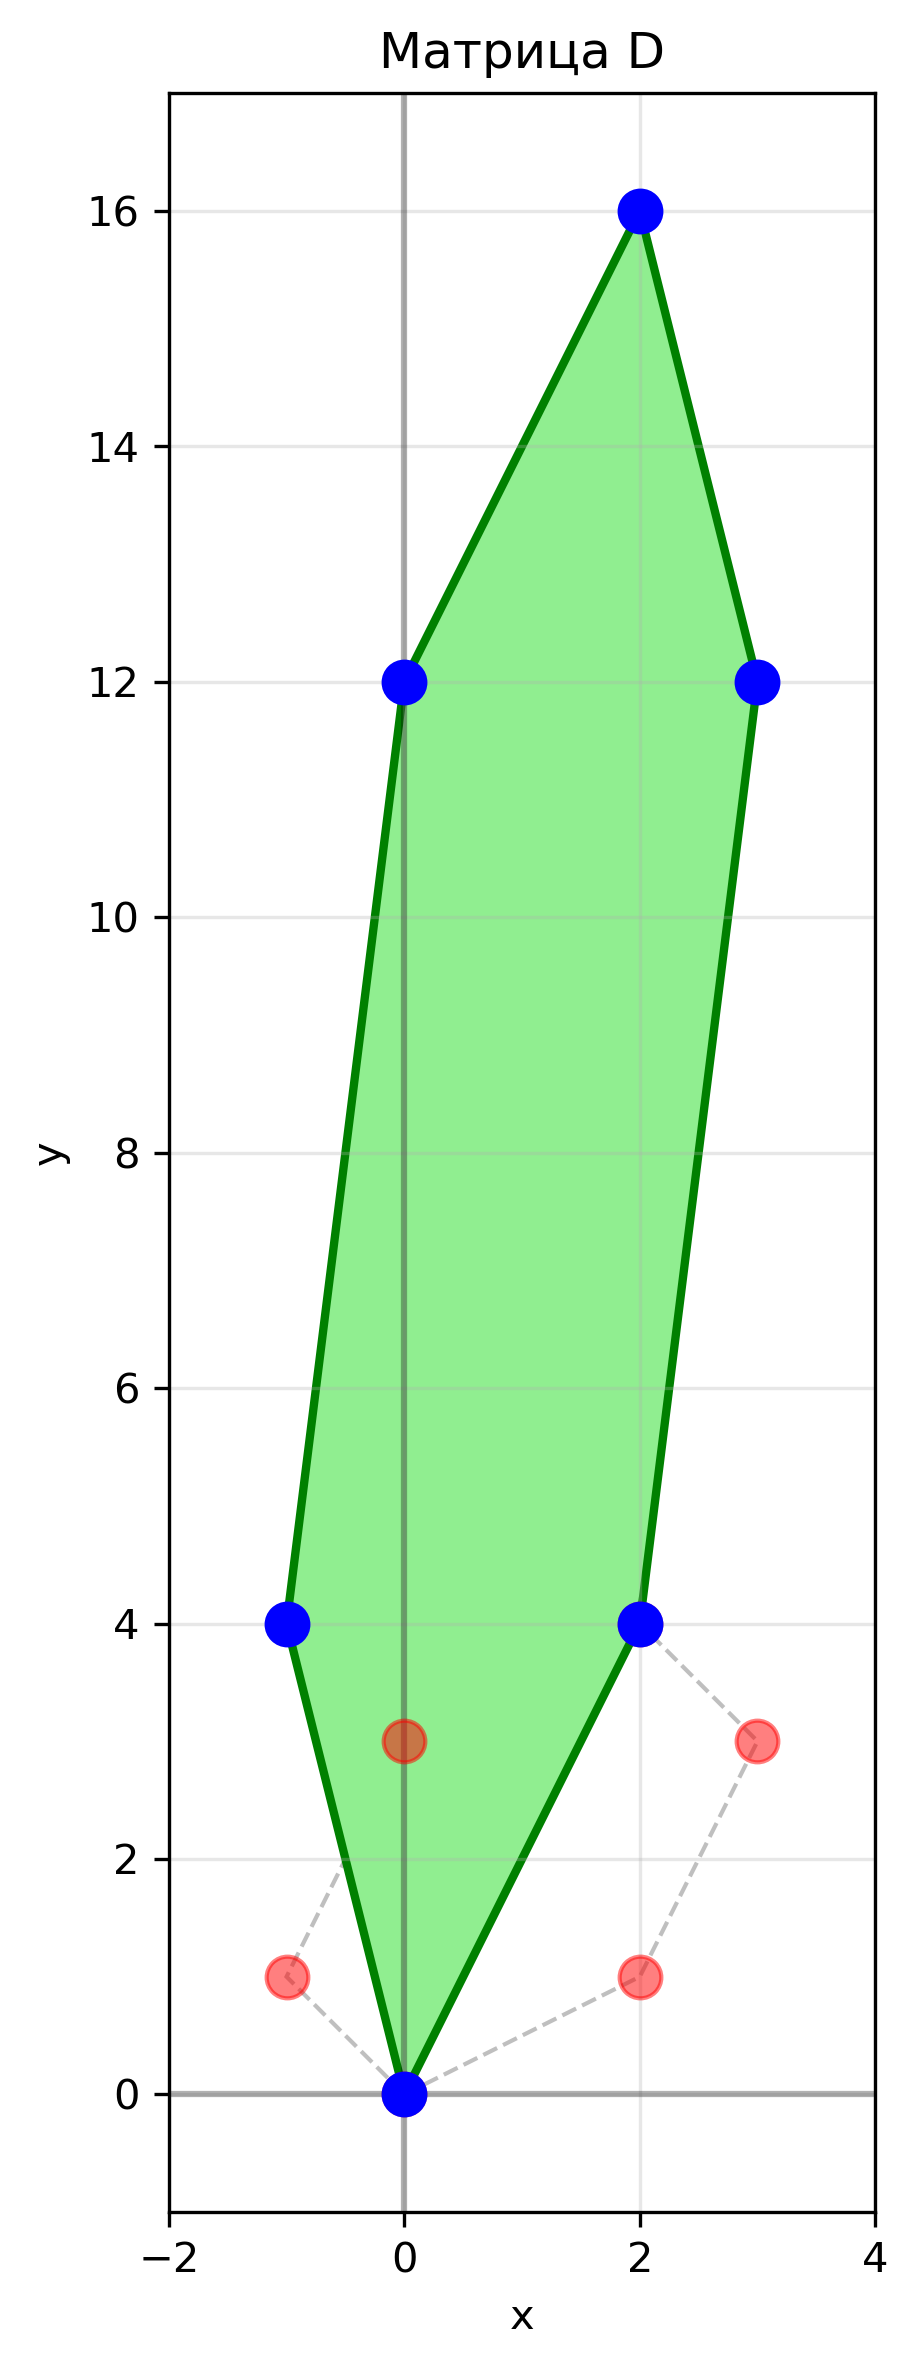
\includegraphics[width=\textwidth]{images/task1/matrix_D.png}
\caption{Матрица $D$}
\label{fig:matrix_D}
\end{minipage}
\hfill
\begin{minipage}{0.23\textwidth}
\centering
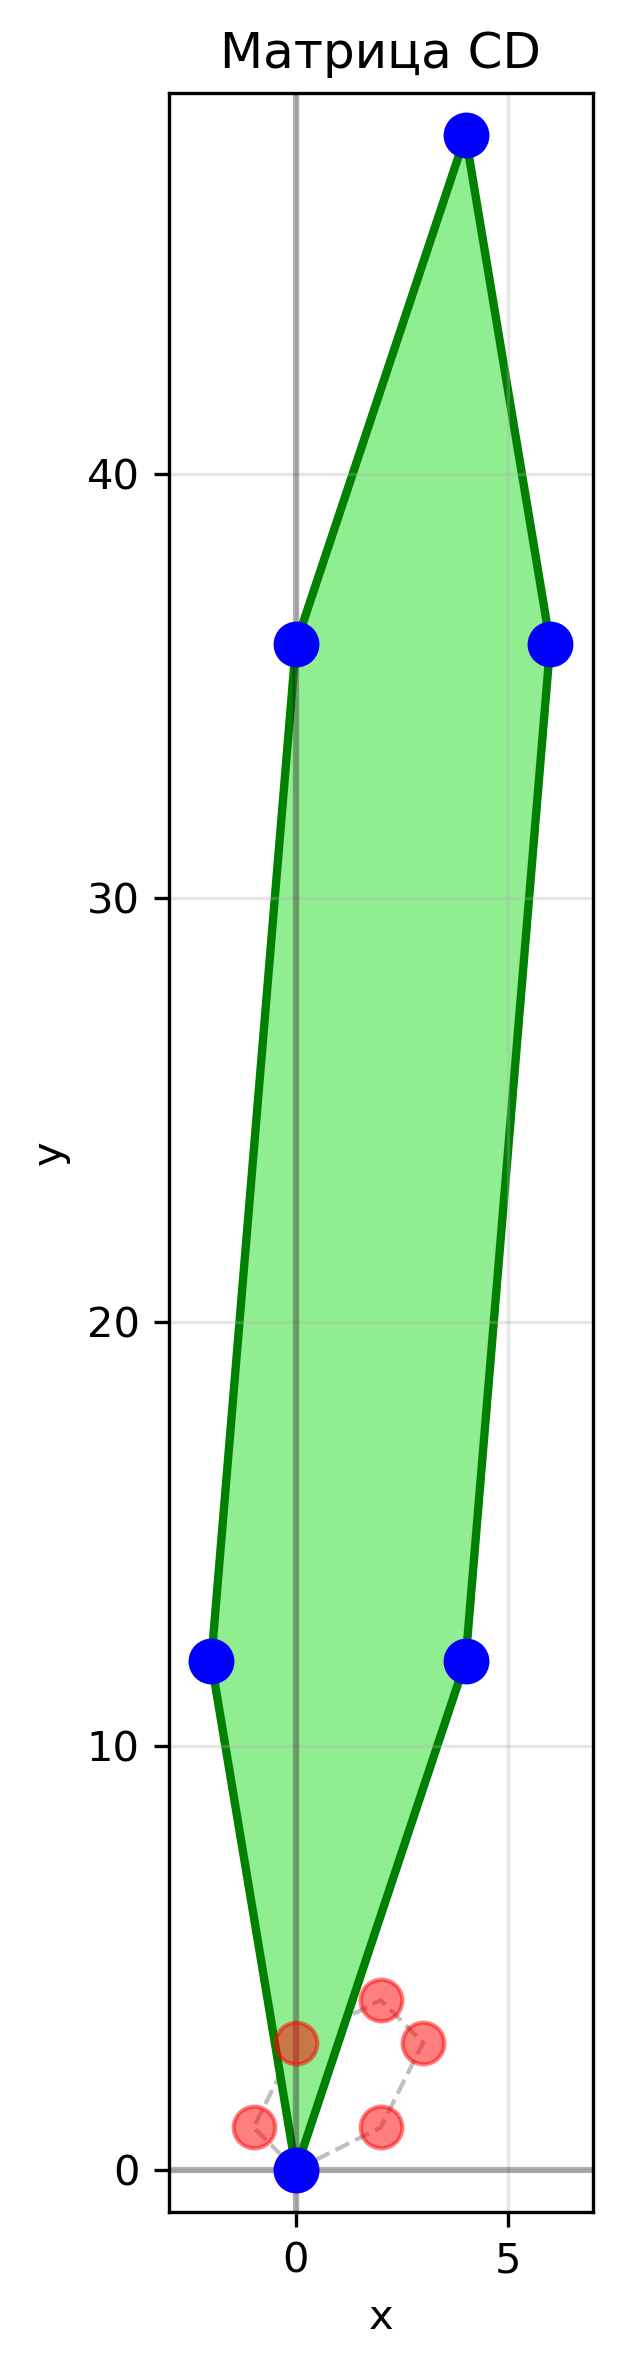
\includegraphics[width=\textwidth]{images/task1/matrix_CD.png}
\caption{Матрица $CD$}
\label{fig:matrix_CD}
\end{minipage}
\hfill
\begin{minipage}{0.23\textwidth}
\centering
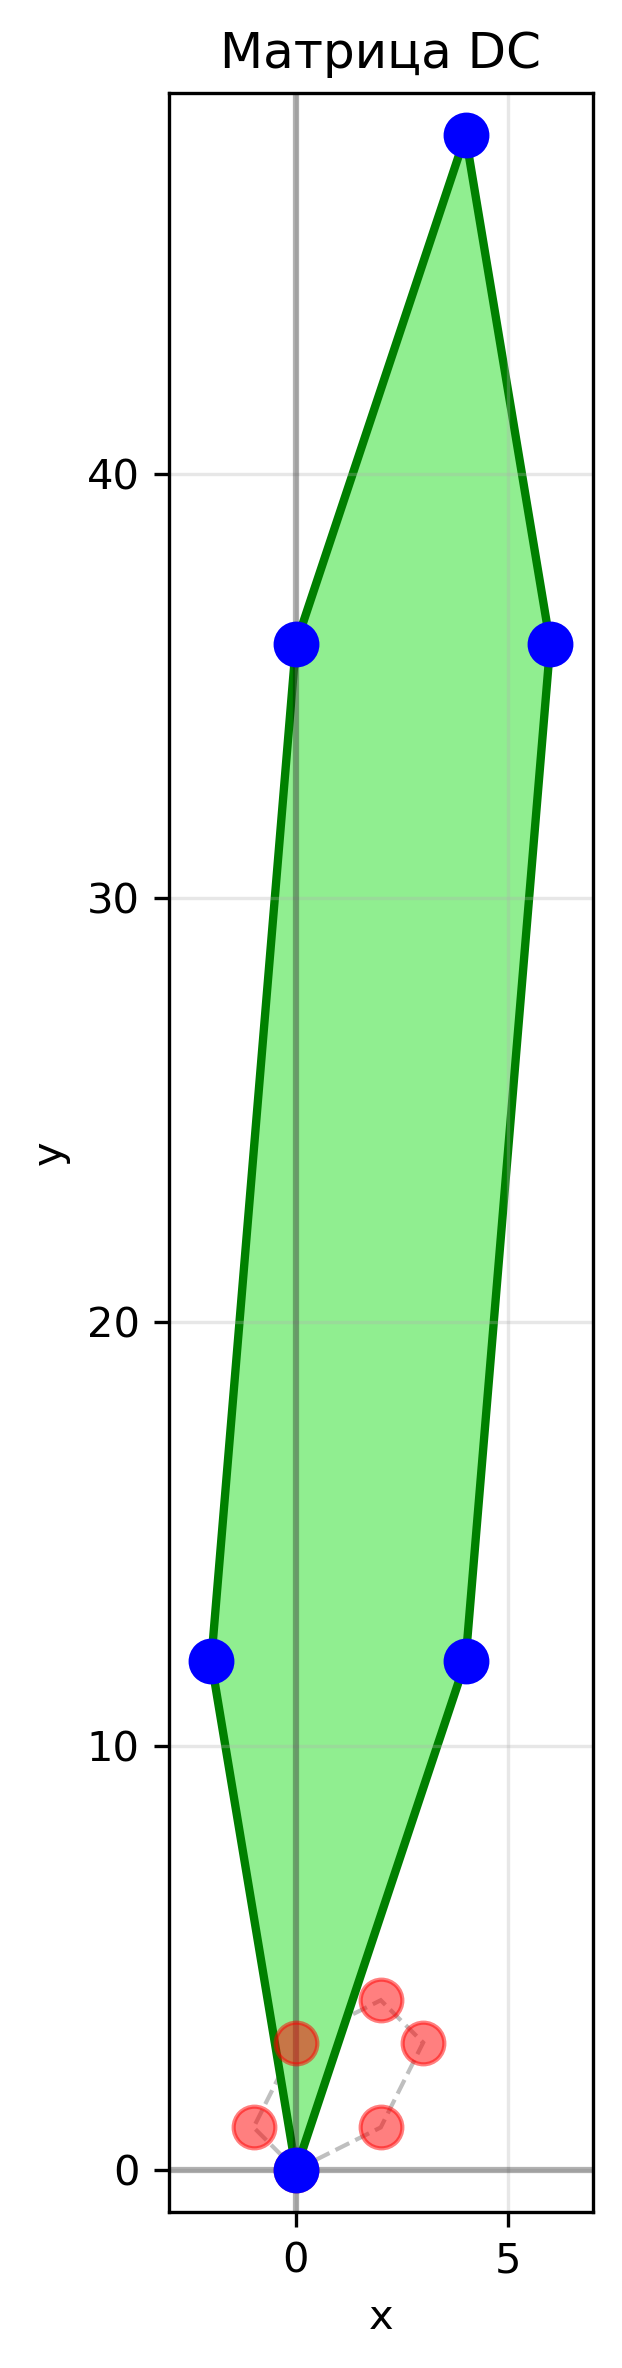
\includegraphics[width=\textwidth]{images/task1/matrix_DC.png}
\caption{Матрица $DC$}
\label{fig:matrix_DC}
\end{minipage}
\end{figure}

\section*{Задание 2: Анализ матричных преобразований}

В данном разделе проводится анализ созданных матричных преобразований: вычисляются образы и ядра, собственные значения и векторы, определители, а также исследуется симметричность матриц.

\subsection*{Анализ образов и ядер}

\subsubsection*{Отражение относительно прямой $y = ax$ (пункт 1)}

\begin{itemize}
\item \textbf{Определитель}: $\det(A_1) = -1.0$
\item \textbf{Ранг}: $\text{rank}(A_1) = 2$
\item \textbf{Собственные значения}: $\lambda_1 = -1$, $\lambda_2 = 1$
\item \textbf{Ядро}: $\text{Ker}(A_1) = \{0\}$ (только нулевой вектор)
\item \textbf{Образ}: $\text{Im}(A_1) = \mathbb{R}^2$ (вся плоскость)
\end{itemize}

Матрица отражения невырождена, поэтому ядро тривиально, а образ совпадает со всей плоскостью.

\subsubsection*{Проекция на прямую $y = bx$ (пункт 2)}

\begin{itemize}
\item \textbf{Определитель}: $\det(A_2) = 0.0$
\item \textbf{Ранг}: $\text{rank}(A_2) = 1$
\item \textbf{Собственные значения}: $\lambda_1 = 0$, $\lambda_2 = 0$ (кратное)
\item \textbf{Ядро}: $\text{Ker}(A_2)$ - нетривиальное (матрица вырождена)
\item \textbf{Образ}: $\text{Im}(A_2)$ - прямая $y = 5x$
\end{itemize}

Матрица проекции вырождена, поэтому ядро нетривиально, а образ представляет собой прямую.

\subsubsection*{Матрица с комплексными собственными значениями (пункт 13)}

\begin{itemize}
\item \textbf{Определитель}: $\det(A_{13}) = 1.0$
\item \textbf{Ранг}: $\text{rank}(A_{13}) = 2$
\item \textbf{Собственные значения}: $\lambda_1 = i$, $\lambda_2 = -i$ (чисто мнимые)
\item \textbf{Ядро}: $\text{Ker}(A_{13}) = \{0\}$ (только нулевой вектор)
\item \textbf{Образ}: $\text{Im}(A_{13}) = \mathbb{R}^2$ (вся плоскость)
\end{itemize}

Несмотря на комплексные собственные значения, матрица невырождена, поэтому ядро тривиально.

\subsubsection*{Скалярное отображение (пункт 14)}

\begin{itemize}
\item \textbf{Определитель}: $\det(A_{14}) = 4.0$
\item \textbf{Ранг}: $\text{rank}(A_{14}) = 2$
\item \textbf{Собственные значения}: $\lambda_1 = 2$, $\lambda_2 = 2$ (кратное)
\item \textbf{Ядро}: $\text{Ker}(A_{14}) = \{0\}$ (только нулевой вектор)
\item \textbf{Образ}: $\text{Im}(A_{14}) = \mathbb{R}^2$ (вся плоскость)
\end{itemize}

Скалярная матрица невырождена, поэтому ядро тривиально, а образ совпадает со всей плоскостью.

\subsection*{Анализ собственных значений и векторов}

Результаты анализа собственных значений для всех матриц:

\begin{itemize}
\item \textbf{Отражение}: $\lambda = [-1, 1]$ - вещественные, различные
\item \textbf{Проекция}: $\lambda = [0, 0]$ - кратные нулевые
\item \textbf{Поворот}: $\lambda = [0.342 + 0.940i, 0.342 - 0.940i]$ - комплексные
\item \textbf{Центральная симметрия}: $\lambda = [-1, -1]$ - кратные отрицательные
\item \textbf{Обмен прямых}: $\lambda = [1.667, 0.6]$ - вещественные, различные
\item \textbf{Перпендикулярные собственные векторы}: $\lambda = [1.382, 3.618]$ - вещественные, различные
\item \textbf{Без двух неколлинеарных собственных векторов}: $\lambda = [2, 2]$ - кратные
\item \textbf{Комплексные собственные значения}: $\lambda = [i, -i]$ - чисто мнимые
\item \textbf{Скалярное отображение}: $\lambda = [2, 2]$ - кратные
\item \textbf{Матрица A (некоммутативные)}: $\lambda = [1, 1]$ - кратные
\item \textbf{Матрица B (некоммутативные)}: $\lambda = [1, 1]$ - кратные
\item \textbf{Матрица C (коммутативные)}: $\lambda = [2, 3]$ - вещественные, различные
\item \textbf{Матрица D (коммутативные)}: $\lambda = [1, 4]$ - вещественные, различные
\end{itemize}

\subsection*{Анализ определителей}

Результаты вычисления определителей для указанных матриц:

\begin{itemize}
\item \textbf{Отражение}: $\det = -1.0000$
\item \textbf{Проекция}: $\det = 0.0000$
\item \textbf{Поворот}: $\det = 1.0000$
\item \textbf{Центральная симметрия}: $\det = 1.0000$
\item \textbf{Отражение + поворот}: $\det = -1.0000$
\item \textbf{Масштабирование}: $\det = 7.0000$
\item \textbf{Эллиптическое преобразование}: $\det = 1.0000$
\end{itemize}

Интересные наблюдения:
\begin{itemize}
\item Определитель отражения равен $-1$, что характерно для ортогональных преобразований с отрицательным определителем
\item Определитель проекции равен $0$, что указывает на вырожденность преобразования
\item Определитель поворота равен $1$, что характерно для ортогональных преобразований
\item Определитель масштабирования равен $7$, что соответствует площади преобразованного круга
\end{itemize}

\subsection*{Анализ симметричности матриц}

Результаты проверки симметричности матриц:

\begin{itemize}
\item \textbf{Отражение}: симметрична
\item \textbf{Проекция}: несимметрична
\item \textbf{Поворот}: несимметрична
\item \textbf{Центральная симметрия}: симметрична
\item \textbf{Обмен прямых}: симметрична
\item \textbf{Перпендикулярные собственные векторы}: симметрична
\item \textbf{Без двух неколлинеарных собственных векторов}: несимметрична
\item \textbf{Комплексные собственные значения}: несимметрична
\item \textbf{Скалярное отображение}: симметрична
\item \textbf{Матрица A (некоммутативные)}: несимметрична
\item \textbf{Матрица B (некоммутативные)}: несимметрична
\item \textbf{Матрица C (коммутативные)}: симметрична
\item \textbf{Матрица D (коммутативные)}: симметрична
\end{itemize}

\subsection*{Ответы на вопросы задания}

\textbf{В каких пунктах матрица обязательно получается симметричной?}

Матрица обязательно получается симметричной в следующих пунктах:

\begin{enumerate}
\item \textbf{Пункт 1} (отражение) - матрица отражения относительно прямой всегда симметрична
\item \textbf{Пункт 4} (центральная симметрия) - диагональная матрица с одинаковыми элементами
\item \textbf{Пункт 8} (обмен прямых) - диагональная матрица
\item \textbf{Пункт 11} (перпендикулярные собственные векторы) - специально построена как симметричная
\item \textbf{Пункт 14} (скалярное отображение) - диагональная матрица с одинаковыми элементами
\item \textbf{Пункт 16} (коммутативные матрицы C и D) - диагональные матрицы
\end{enumerate}

Общий принцип: симметричными получаются матрицы, которые либо являются диагональными, либо специально построены как симметричные для получения перпендикулярных собственных векторов.

\section*{Заключение}

В ходе выполнения лабораторной работы №2 были успешно созданы и проанализированы 16 различных матричных преобразований $2 \times 2$, каждое из которых демонстрирует уникальные свойства линейных отображений плоскости.

\subsection*{Основные результаты}

\begin{enumerate}
\item \textbf{Созданы матрицы} для всех требуемых типов преобразований: отражения, проекции, повороты, симметрии, масштабирования и других
\item \textbf{Выполнена визуализация} всех преобразований с помощью многоугольника, что позволило наглядно увидеть действие каждого преобразования
\item \textbf{Проведен анализ} собственных значений и векторов, определителей, образов и ядер матриц
\item \textbf{Исследована коммутативность} матричного умножения на примерах пар матриц
\item \textbf{Выявлены закономерности} в симметричности матриц различных типов преобразований
\end{enumerate}

\subsection*{Ключевые выводы}

\begin{itemize}
\item \textbf{Ортогональные преобразования} (отражения, повороты) имеют определитель $\pm 1$
\item \textbf{Вырожденные преобразования} (проекции) имеют определитель $0$ и нетривиальное ядро
\item \textbf{Симметричные матрицы} имеют вещественные собственные значения и ортогональные собственные векторы
\item \textbf{Комплексные собственные значения} возникают у матриц поворота и некоторых других преобразований
\item \textbf{Коммутативность матричного умножения} не является общим свойством и зависит от конкретных матриц
\end{itemize}

\subsection*{Практическая значимость}

Полученные результаты имеют важное значение для понимания:
\begin{itemize}
\item Геометрических преобразований в компьютерной графике
\item Линейной алгебры и теории матриц
\item Применения матричных методов в различных областях науки и техники
\end{itemize}

Лабораторная работа успешно выполнена, все задания решены с подробным анализом и визуализацией результатов.
